\documentclass[11pt]{article}

% general packages without options
\usepackage{amsmath,amssymb,bbm,amsfonts,amsthm}
\usepackage{commath}
% graphics
\usepackage{graphicx}
% text formatting
\usepackage[document]{ragged2e}
\usepackage{pagecolor,color}

\newcommand{\noun}[1]{\textsc{#1}}

\usepackage[utf8]{inputenc}
\usepackage[T1]{fontenc}
% geometry
\usepackage[margin=1.8cm]{geometry}

\usepackage{multicol}
\usepackage{setspace}



\usepackage{natbib}
\setlength{\bibsep}{0.0pt}

\usepackage[french]{babel}

% layout : use fancyhdr package
%\usepackage{fancyhdr}
%\pagestyle{fancy}

% variable to include comments or not in the compilation ; set to 1 to include
\def \draft {1}


% writing utilities

% comments and responses
%  -> use this comment to ask questions on what other wrote/answer questions with optional arguments (up to 4 answers)
\usepackage{xparse}
\usepackage{ifthen}
\DeclareDocumentCommand{\comment}{m o o o o}
{\ifthenelse{\draft=1}{
    \textcolor{red}{\textbf{C : }#1}
    \IfValueT{#2}{\textcolor{blue}{\textbf{A1 : }#2}}
    \IfValueT{#3}{\textcolor{ForestGreen}{\textbf{A2 : }#3}}
    \IfValueT{#4}{\textcolor{red!50!blue}{\textbf{A3 : }#4}}
    \IfValueT{#5}{\textcolor{Aquamarine}{\textbf{A4 : }#5}}
 }{}
}

% todo
\newcommand{\todo}[1]{
\ifthenelse{\draft=1}{\textcolor{red!50!blue}{\textbf{TODO : \textit{#1}}}}{}
}


\makeatletter


\makeatother


\begin{document}







\title{Espace et complexités des systèmes territoriaux
\\\bigskip
\textit{Actes des Journ{\'e}es de Rochebrune 2019}
}
\author{\noun{Juste Raimbault}$^{1,2,3}$
\bigskip\\
$^1$ UPS CNRS 3611 ISC-PIF\\
$^2$ CASA, UCL\\
$^3$ UMR CNRS 8504 G{\'e}ographie-cit{\'e}s
}
\date{}


%\pagenumbering{gobble}



\maketitle

\justify

\begin{abstract}
	Le caractère spatialisé des systèmes territoriaux joue un rôle déterminant dans l'émergence de leurs complexités. Cette contribution vise à illustrer dans quelle mesure différents types de complexités peuvent se manifester dans des modèles de tels systèmes. Nous développons d'un point de vue théorique des arguments illustrant la complexité ontologique, au sens de la multitude et multidimensionalité de représentations possibles, puis la complexité au sens de l'émergence, c'est-à-dire la nécessité de l'existence de plusieurs niveaux autonomes. Nous proposons ensuite des expériences numériques pour explorer des propriétés de la complexité (complexité dynamique et co-évolution) au sein de deux modèles simples de morphogenèse urbaine. Nous suggérons finalement d'autres dimensions de la complexité qui pourraient être typiques des systèmes territoriaux.\medskip\\
	\noindent\textbf{Mots-clés : }\textit{Complexités; Systèmes territoriaux; Morphogenèse urbaine; Co-évolution}
\end{abstract}





\added{\cite{Aubry1991}}


\section{Introduction}


Les systèmes territoriaux, qui peuvent être compris comme des structures socio-spatiales auto-organisées \citep{pumain1997pour}, sont une illustration typique de systèmes complexes étudiés sous de nombreux angles incluant plus ou moins l'aspect spatial de ces systèmes. Notre appréhension des systèmes territoriaux se place plus particulièrement dans la lignée de la théorie évolutive des villes~\citep{pumain2018evolutionary} qui comprend les systèmes urbains comme des systèmes multi-niveaux, dans lesquels la co-évolution des multiples composants et agents détermine la dynamique de ceux-ci~\citep{raimbault2018caracterisation}. La complexité de ces systèmes est ainsi étroitement liée à leur caractère spatial, puisque leurs dynamiques sont portées par les distributions spatiales de leur entités et sous-systèmes, et que les interactions entre agents conduisant au comportement émergent sont inscrites dans l'espace.

Le concept de complexité correspond à de diverses approches et définitions, qui dépendent des domaines où elles sont introduites. Par exemple, \cite{chu2008criteria} passe en revue les approches conceptuelles et opérationnelles liées au champ de la vie artificielle et montre qu'il n'existe pas de concept unifié. \cite{deffuant2015visions} développe aussi différentes visions de la complexité, allant d'une complexité proche d'une complexité computationnelle à une complexité irréductible propre aux systèmes sociaux. Un précédent travail par \cite{raimbault2018relating} s'était proposé de suggérer des ponts épistémologiques entre différentes approches et définitions de la complexité, et plus particulièrement les liens entre complexité au sens d'émergence, complexité computationnelle et complexité informationnelle. Comme le souligne \cite{batty2018defining}, les dimensions de la complexité sont potentiellement infinies et il ne peut exister d'approche universellement valide pour l'ensemble des problèmes et systèmes. Il est alors important de combiner différentes approches de la complexité pour comprendre son rôle au sein des systèmes territoriaux. 

Cette contribution vise à illustrer une approche des systèmes territoriaux par la géographie urbaine, et dans quelle mesure leur complexité est intimement liée à leur caractère spatial. Nous tâchons ici d'illustrer les liens entre complexité et espace selon différentes vues de celle-ci, à la fois à travers des considérations théoriques mais aussi par l'exploration de modèles de simulation de systèmes territoriaux. La suite de cet article est organisée de la façon suivante : dans deux premières sections nous développons une approche conceptuelle de la complexité ontologique et de l'émergence au sein des systèmes territoriaux. Nous présentons ensuite des résultats de simulation d'un modèle de morphogenèse urbaine exhibant des propriétés typiques de la complexité dynamique. Une autre expérience permet ensuite de montrer le lien entre complexité au sens d'une co-évolution et la structure spatiale du système. Nous discutons finalement les implications des ces résultats et des développements possibles.



%%%%%%%%%%%%%%%%%
\section{Complexité ontologique}
%%%%%%%%%%%%%%%%%


%%%%%%%%%%%%%%%%%
%\subsection{Multidimensionalité et diversité d'approches}


Une première approche théorique permet une entrée sur ce que nous appelons \emph{complexité ontologique}, qui a été proposée par \cite{pumain2003approche} comme la largeur des points de vue disciplinaires nécessaires pour appréhender un même objet. La multidimensionalité des systèmes territoriaux reste un enjeu principal pour leur compréhension, comme l'illustre \cite{perez2016agent} dans le cas des systèmes multi-agents. Ainsi, l'interdisciplinarité serait intrinsèque aux ``sciences urbaines'', c'est-à-dire aux différentes disciplines prenant la ville comme objet d'étude, même si celle-ci s'avère en pratique laborieuse et soumise à la contingence de l'organisation sociale des sciences \citep{dupuy2015sciences}.


Nous reprenons l'exemple de \cite{raimbault2017invisible} comme preuve-de-concept de la diversité des approches possibles dans le cas des relations entre réseaux et territoires, et suggérons des pistes de réflexion quant au rôle de l'espace dans cette complexité, comme les processus évolutifs de diversification ou de spécialisation liés aux niches spatiales. Plus précisément, \cite{raimbault2017invisible} établit une cartographie scientifique des approches de modélisation des interactions entre réseaux de transport et territoires. Par une étude de réseaux de citations, émergent des approches complémentaires, incluant par exemple la géographie quantitative, la géographie politique, l'économie urbaine, la planification, la physique. Chaque approche éclaire sur une dimension particulière du même système. L'espace permettant la différentiation des sous-systèmes, il parait d'une part naturel que certains soient plus saillants que d'autres sur les différentes instances, et d'autre part que des interrogations complémentaires cohabitent (celles-ci étant en fait endogènes aux systèmes territoriaux, puisque l'innovation et donc la recherche et la science sont un moteur important des dynamiques des systèmes urbains \citep{pumain2010theorie}).




%%%%%%%%%%%%%%%%%
%\subsection{L'espace porteur de richesse ontologique ?}

À ce point, nous proposons une hypothèse, dont l'exploration empirique nécessiterait des analyses scientométriques poussées hors de portée de ce travail, selon laquelle une spatialisation plus élaborée serait lié à un éventail ontologique plus large. L'exemple de la \emph{New Economic Geography} et de la géographie économique illustre ce cas \citep{marchionni2004geographical}: la première approche, afin de déployer ses outils analytiques, impose un réductionnisme puissant sur l'espace (ligne ou cercle pour une grande partie des modèles) et sur les objets (agents représentatifs, homogénéité), tandis que la seconde favorisera des descriptions empiriques fidèles aux particularités géographiques. Il est difficile de dire si l'espace est plus riche parce que l'approche n'est pas réductionniste ou le contraire, qu'un espace riche augmente la portée ontologique. Prétendre un sens de causalité serait en fait contre-productif, et cette congruence confirme notre argument qu'une spatialisation élaborée des modèles des systèmes territoriaux va de pair avec une plus grande richesse ontologique.

Cette reflexion peut être poussée sur le plan méthodologique, au sein duquel on peut retrouver la tension entre précision du modèle et robustesse des résultats, notamment en comparant les modèles basés-agent et les modèles de systèmes dynamiques permettant un certain niveau de résolution analytique. L'archétype des approches en géographie économique, considérant un système unidimensionnel \citep{krugman1992dynamic}, perd l'essence de l'espace qui est hétérogénéité et multiplicité des alternatives, tandis que des modèles précisément spatialisés comme les modèles Luti, nécessiteront simulation et une validation restreinte des résultats \citep{bonnel2014survey}. Le degré de précision des modèles n'est cependant pas directement relié à leur caractère spatial, comme le montre la comparaison entre modèles agents et microsimulation démographique \citep{birkin2011spatial}. Cependant, les approches incluant une description élaborée de l'espace, avec la prise en compte des échelles par exemple, sont principalement associées à une richesse ontologique dans l'étude de ces systèmes, qu'il convient d'entretenir pour maintenir la diversité des connaissances sur le sujet \citep{sanders2018survival}.


%%%%%%%%%%%%%%%%
\section{Complexité et émergence}
%%%%%%%%%%%%%%%%



Notre deuxième entrée théorique s'intéresse à la complexité en tant qu'émergence faible de structures et autonomie des niveaux supérieurs~\citep{bedau2002downward}. L'émergence faible consiste en l'interprétation que les niveaux d'un système sont effectivement \emph{computés} \citep{morin1980methode} par celui-ci, et qu'il est nécessaire de simuler le système pour les reproduire. L'aspect diachronique des dynamiques permet que cette vue de l'émergence ne soit pas incompatible avec la causalité descendante. Nous rappelons le caractère intrinsèquement multi-échelle des systèmes territoriaux, qui se manifeste par exemple dans l'approche des villes comme systèmes au sein de systèmes de villes, comme l'introduit \cite{pumain1997pour} qui enrichit \cite{berry1964cities}. Par ailleurs, il existe une nécessité actuelle de production de modèles spatiaux intégrant effectivement cet aspect multi-échelle~\citep{rozenblat2018conclusion}, dans le but de modèles effectivement opérationnels.

La difficulté d'endogénéisation de niveau supérieurs autonomes peut par exemple être illustrée par~\cite{lenechet:halshs-01272236} qui propose un modèle de co-évolution entre transport et usage du sol à l'échelle métropolitaine intégrant une structure de gouvernance endogène pour le réseau de transport. Simulant les négociations entre acteurs locaux du transport, certains régimes conduisent à l'émergence d'un niveau intermédiaire de gouvernance issu de la collaboration entre acteurs voisins. Les trois niveaux décisionnels sont alors bien autonomes ontologiquement mais aussi en termes de dynamiques. L'émergence de la collaboration est finement liée à la structure spatiale, puisque les acteurs incluent les motifs d'accessibilité dans leur processus de prise de décision. Des modèles moins riches de la co-évolution entre transport et usage du sol, comme \cite{raimbault2018urban} à l'échelle mesoscopique prenant en compte forme urbaine et topologie du réseau routier, ou \cite{raimbault2018modeling} qui abstrait les réseaux sous formes de matrices de distance à l'échelle macroscopique et postule des dynamiques sur celles-ci, capturent bien une émergence fondamentalement liée à l'espace, mais restent restreints dans l'articulation des niveaux, tandis que le modèle de gouvernance est plus proche de l'émergence qualitative de niveaux supérieurs.

Des systèmes de complexité ontologique moindre présentent aussi un rôle crucial de l'émergence faible. L'état local d'un flux de trafic est en partie conséquence de l'état global du système, en particulier lorsque des motifs de congestion conséquents sont observables à l'échelle macroscopique. Dans ce cas, les motifs spatio-temporels sont encore cruciaux dans le processus d'émergence \citep{treiber2010three}. Dans ces différents exemples, l'espace joue encore un rôle crucial pour la présence de complexité, puisque l'auto-organisation implique agencement spatial des agents, et les niveaux d'émergence sont directement liés aux échelles spatiales quel que soit l'interprétation de celles-ci \citep{manson2008does}. Une approche de l'auto-organisation par la morphogenèse, que nous détaillerons au sein de modèles par la suite, insiste d'autant plus sur l'aspect spatial dans l'émergence, puisqu'elle fait le lien entre forme et fonction \citep{doursat2012morphogenetic}, la première étant nécessairement spatialisée.






%%%%%%%%%%%%%%%%%
\section{Complexité dynamique}
%%%%%%%%%%%%%%%%%


Dans cette section ainsi que la suivante, nous proposons d'utiliser des modèles de simulation de morphogenèse urbaine pour montrer de manière concrète d'autres complexités des systèmes territoriaux. Les modèles, détaillés par la suite, sont implémentés en Netlogo \citep{wilensky1999netlogo} et en scala, et explorés à l'aide du logiciel d'exploration de modèles OpenMOLE \citep{reuillon2013openmole}. L'ensemble du code et des résultats est disponible de manière ouverte sur le dépôt git du projet à \texttt{https://github.com/JusteRaimbault/SpatialComplexity}. Les résultats de simulation sont disponibles à \texttt{https://doi.org/10.7910/DVN/LENFVH}.


%\subsection{Systèmes dynamiques, chaos et fractales}


La compréhension des systèmes complexes comme systèmes dynamiques aux attracteurs plus ou moins chaotiques a été largement développée en géographie \citep{dauphine1995chaos}. Par exemple, \cite{e18060197} considère que l'information sémantique d'un environnement urbain est liée aux attracteurs de systèmes dynamiques régissant les dynamiques de ses agents. Ce type d'approche peut par ailleurs être rapprochée des approches fractales des systèmes urbains, initialement introduites par \cite{batty1994fractal}, et par exemple plus récemment appliquées à des problèmes réels de planification urbaine \citep{yamu2015spatial}. Ces questions sont liées plus généralement à des problématiques transversales de chaos spatio-temporel \citep{crutchfield1987phenomenology}. La compréhension du lien entre temps et espace, et des dynamiques non-uniformes, non-stationnaires, non-ergodiques correspondantes, reste en construction sur les plans théoriques, méthodologique et empirique, et promet de nombreuses applications pour l'étude des systèmes territoriaux. Par exemple,  \cite{chen2009urban} combine les correlations croisées et l'analyse de Fourier pour étudier un modèle de gravité urbaine. Une direction de recherche importante dans ce cadre est la compréhension de la non-stationnarité des propriétés des systèmes territoriaux, et \cite{raimbault2018urban} l'explore dans le cas de la morphologie urbaine et de la forme des réseaux.




%\subsection{Sensibilité aux conditions initiales et dépendance au chemin}

Nous utilisons ici un modèle de morphogenèse urbaine introduit par \cite{raimbault2018calibration} pour illustrer les propriétés de sensibilité aux conditions initiales et de dépendance au chemin des systèmes territoriaux~\citep{pumain2012urban}. En particulier, nous montrons la forte sensibilité des formes urbaines finales simulées aux perturbations spatiales, et plus généralement la dépendance au chemin des trajectoires pour les indicateurs morphologiques agrégés. Ce modèle relativement simple simule la croissance de population distribuée sur une grille, par ajout itératif de population, qui se localise suivant un attachement préférentiel à la population déjà présente puis se diffuse dans l'espace. Les paramètres cruciaux sont $N_G$ le taux de croissance exogène, $P_{max}$ la population totale finale, $\alpha$ l'exposant d'attachement préférentiel, $\beta$ le taux de diffusion et $n_d$ un nombre de diffusions par pas de temps.

L'experience menée par \cite{raimbault2018calibration} sur une version simplifiée à une dimension du modèle montre que les distributions semi-stationnaires de population peuvent être à distance maximale (au sens d'une norme L2 entre les distributions) à partir d'une même configuration initiale. En deux dimensions, le phénomène est identique comme l'expérience menée ici le montre. Le modèle est simulé à partir d'une configuration initiale particulièrement sensible, constituée de 4 centres initiaux de taille équivalente. Pour une grille de taille 100, 4 centres sont positionnés au milieu de chaque cadrant, avec un noyau exponentiel de population de la forme $P_0 \cdot \exp \left(-r/r_0\right)$ avec $P_0 = 100$ et $r_0 = 5$. Le modèle est alors simulé pour des valeurs données des paramètres d'agrégation $\alpha$, de diffusion $\beta, n_d$, de croissance et population $N_G, P_{max}$ (voir \cite{raimbault2018calibration}), et une réalisation de la distance entre configuration $d(t)$ est calculée sur deux réalisations indépendantes des populations $P^{(k)}_i(t)$, comme $d(t)=\norm{P^{(1)}_i(t) - P^{(2)}_i(t)}$. Un plan d'expérience direct est effectué, par échantillonnage LHS de 390 points de paramètres et 1000 répétitions.



%      adjr2           lambda1           lambda2               ids             id           alpha       
% Min.   :0.5332   Min.   :0.05242   Min.   :0.0009514   Min.   :2382   Min.   :2382   Min.   :0.5016  
% 1st Qu.:0.9261   1st Qu.:0.14034   1st Qu.:0.0091442   1st Qu.:2974   1st Qu.:2974   1st Qu.:0.9059  
% Median :0.9555   Median :0.25679   Median :0.0148210   Median :3458   Median :3458   Median :1.4044  
% Mean   :0.9372   Mean   :0.31340   Mean   :0.0220534   Mean   :3454   Mean   :3454   Mean   :1.4210  
% 3rd Qu.:0.9722   3rd Qu.:0.44971   3rd Qu.:0.0275092   3rd Qu.:3963   3rd Qu.:3963   3rd Qu.:1.9154  
% Max.   :0.9888   Max.   :0.84750   Max.   :0.2040800   Max.   :4407   Max.   :4407   Max.   :2.4924  
 %     beta                 nd        relgrowthrate        growthrate      population   
% Min.   :0.0001532   Min.   :1.003   Min.   :0.005373   Min.   :500.5   Min.   :10285  
% 1st Qu.:0.1129967   1st Qu.:1.947   1st Qu.:0.010791   1st Qu.:631.5   1st Qu.:30425  
% Median :0.2408924   Median :2.884   Median :0.014974   Median :764.0   Median :50103  
% Mean   :0.2420500   Mean   :2.952   Mean   :0.019731   Mean   :761.0   Mean   :51729  
% 3rd Qu.:0.3665757   3rd Qu.:3.959   3rd Qu.:0.024075   3rd Qu.:886.5   3rd Qu.:70556  
% Max.   :0.4999998   Max.   :4.999   Max.   :0.086181   Max.   :999.7   Max.   :99790
%summary(breaks)
%   Min. 1st Qu.  Median    Mean 3rd Qu.    Max. 
%  2.492   6.947   9.389  10.701  12.732  37.020 

Nous montrons en Fig.~\ref{fig:lyapounov} une estimation basique des exposants de Lyapounov, effectuée par ajustement par régression linéaire par morceaux avec deux segments, de $\log d(t)$ en fonction de $t$, sur l'ensemble des répétitions pour un point de paramètres. L'ajustement est relativement bon puisque le premier quartile du $R^2$ ajusté est à 0.92 et sa moyenne à 0.93. L'exposant de Lyapounov sur le premier segment, qu'on note $\lambda_1$, varie entre 0.05 et 0.84 avec une moyenne de 0.31. Ainsi, la qualité de l'ajustement et les valeurs positives montrent la forte sensibilité aux conditions initiales des configurations générées. Les régimes temporels sont assez différents, puisque le temps de rupture $t_b$ estimé varie entre 2.5 et 37.0. Les valeurs de $\lambda_2$ sont plus faibles, avec une moyenne à 0.02. Il existe un premier régime durant lequel le principal de la structure urbaine se constitue puis un deuxième régime (qu'on pourrait qualifier de ``semi-stationnaire'') pendant lequel les évolutions sont plus mineures. Cela suggère par ailleurs un critère d'arrêt endogène au modèle. Les courbes de $\log d(t)$ montrées en Fig.~\ref{fig:lyapounov} sont pour une valeur maximale de l'ajustement et une valeur maximale de $\lambda_1$. Nous montrons aussi les variations des exposants en fonction des paramètres. $\lambda_1$ en fonction de l'agrégation $\alpha$ présente un comportement inattendu, relativement stable en dessous de 1.5 puis une croissance linéaire au dessus, sans modification autour de 1, ce qui suggère un seuil au dessus duquel ce processus influe drastiquement sur la forme urbaine. Pour les plus faibles valeurs de $\beta$, un maximum local à 1 suggère un rôle de l'aspect infra ou supra-linéaire du régime. Pour le comportement de $\lambda_2$, un effet significatif s'observe uniquement pour les plus forts taux de croissance, et correspond à un maximum autour de 1.5, c'est-à-dire que le passage au second régime pour $\lambda_1$ correspond dans ce cas à une meilleure stabilisation pour la seconde phase. Cette étude montre donc la sensibilité des configurations urbaines à des perturbations infinitésimales (ce qui est est équivalent à une perturbation de l'état initial).



%%%%%%%%%%%%%
\begin{figure}
	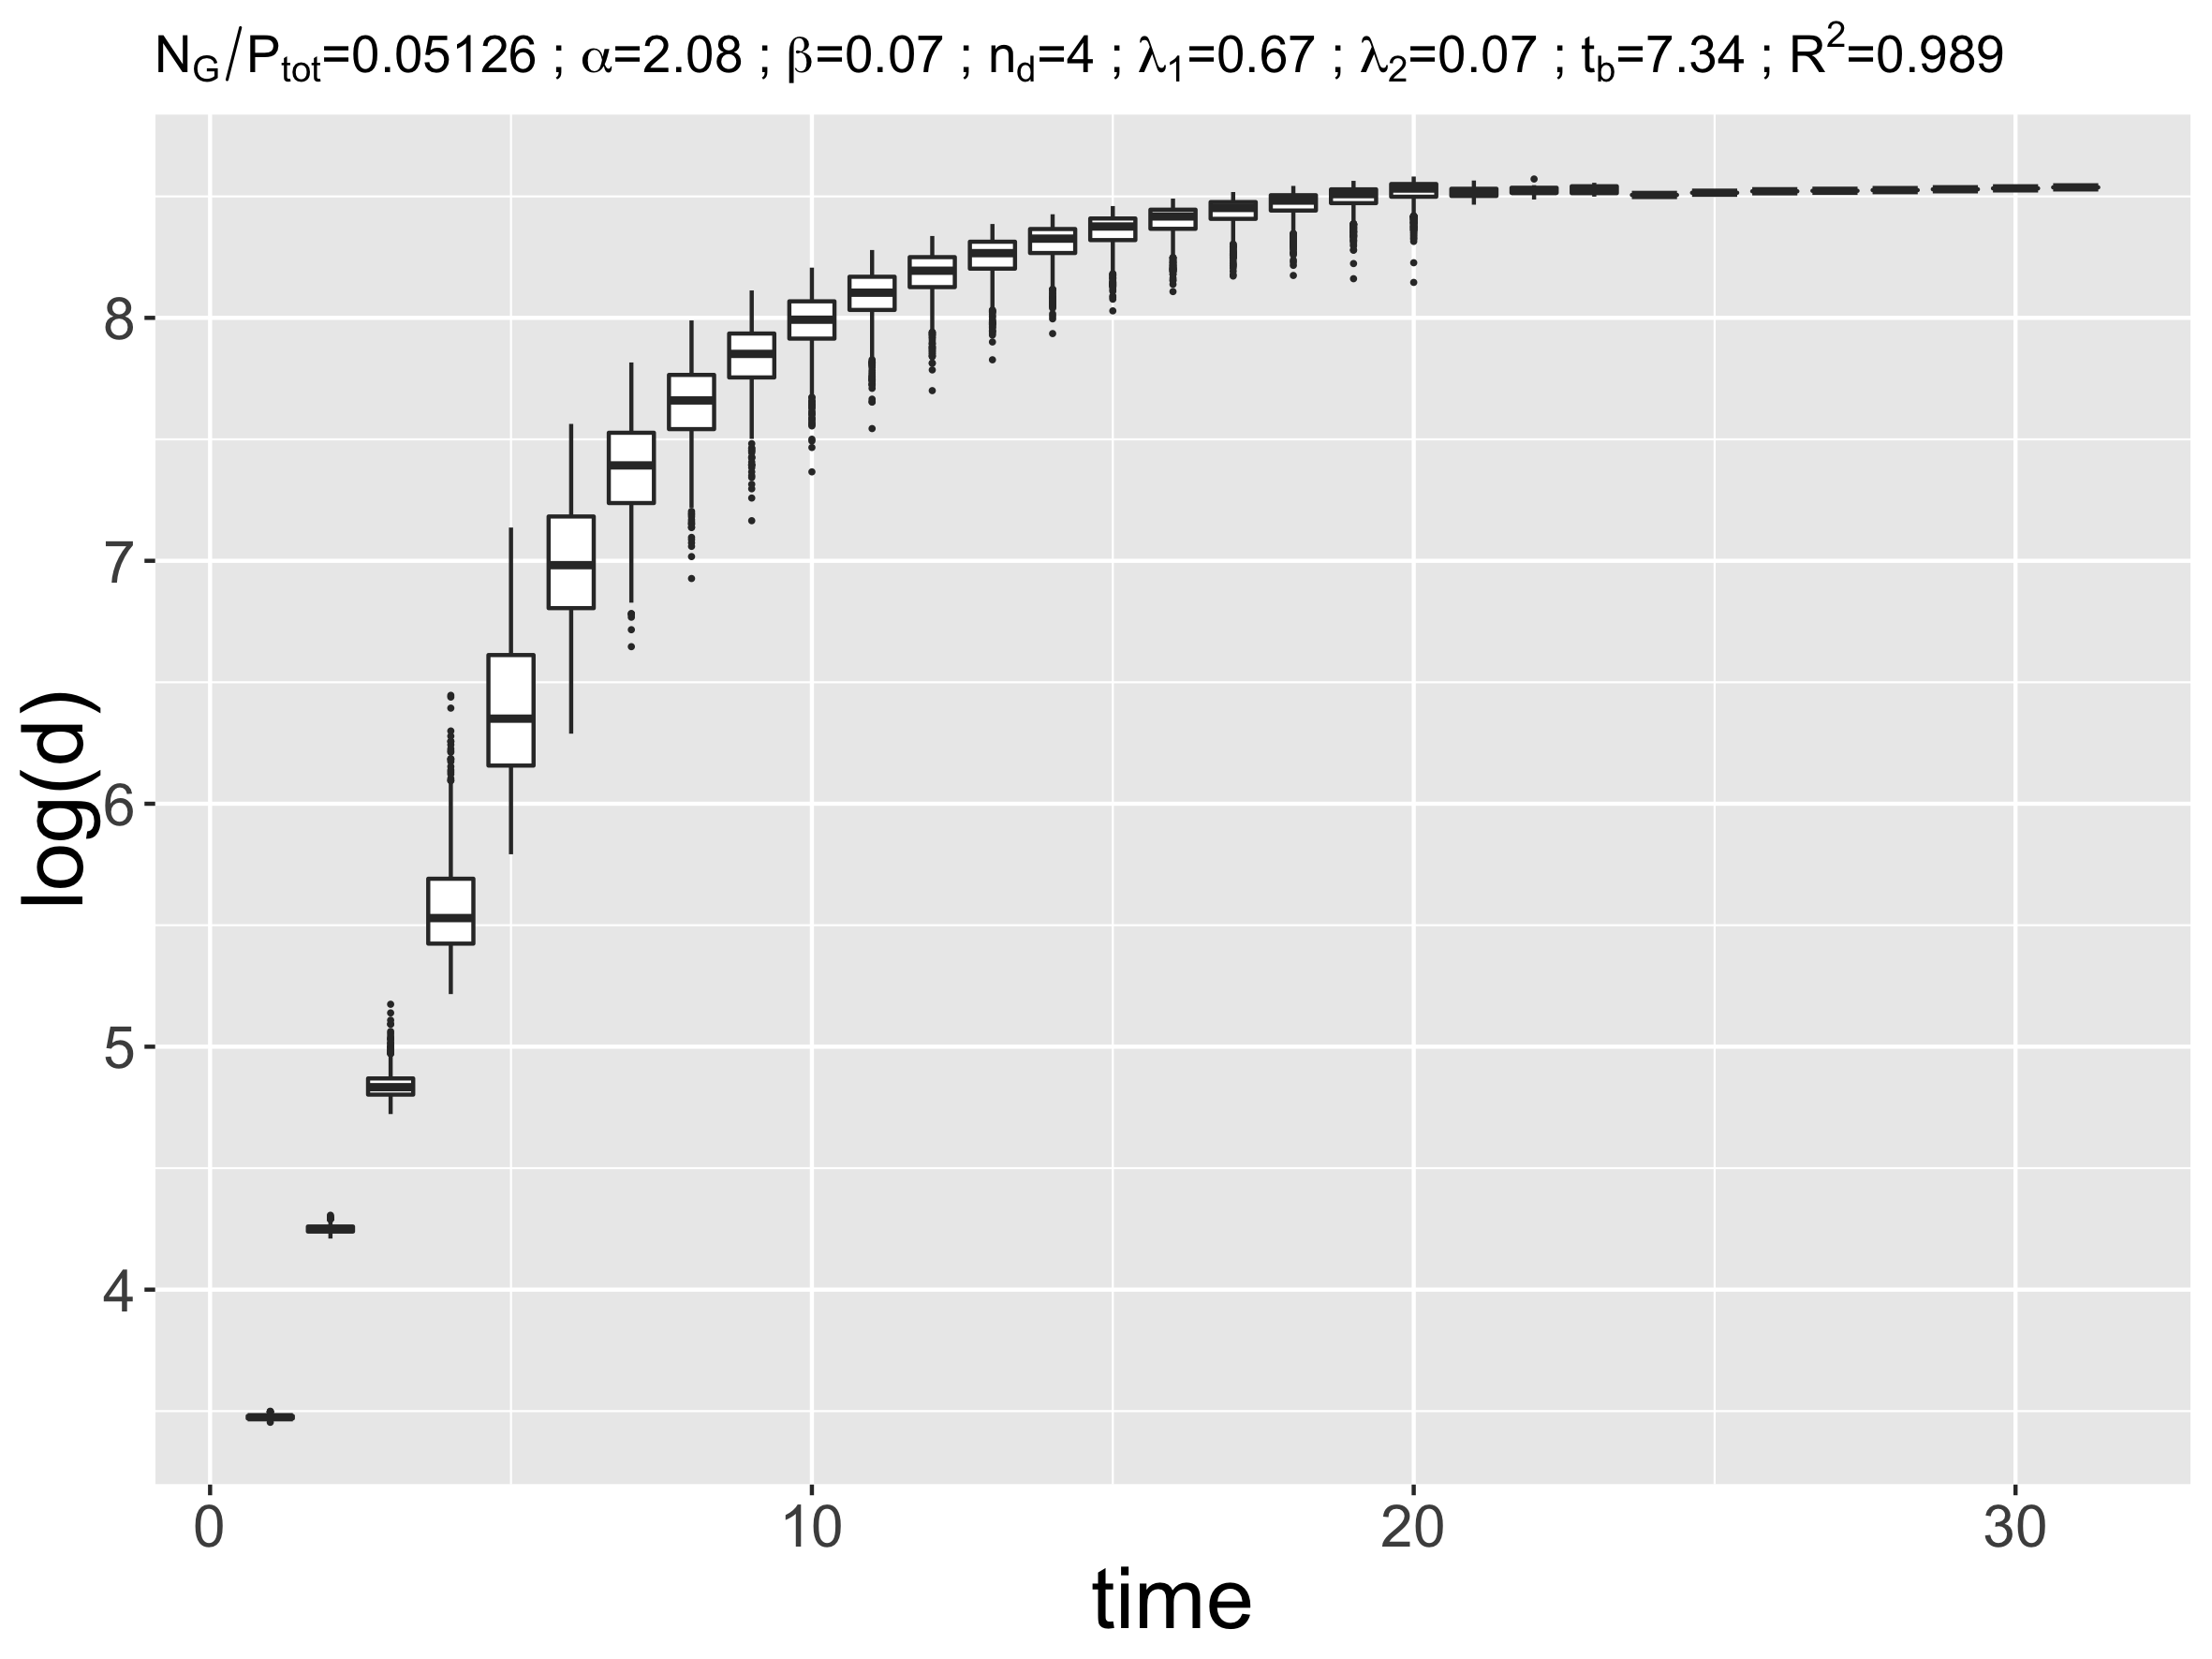
\includegraphics[width=0.49\linewidth]{figures/configdist_boxplot_id3642.png}
	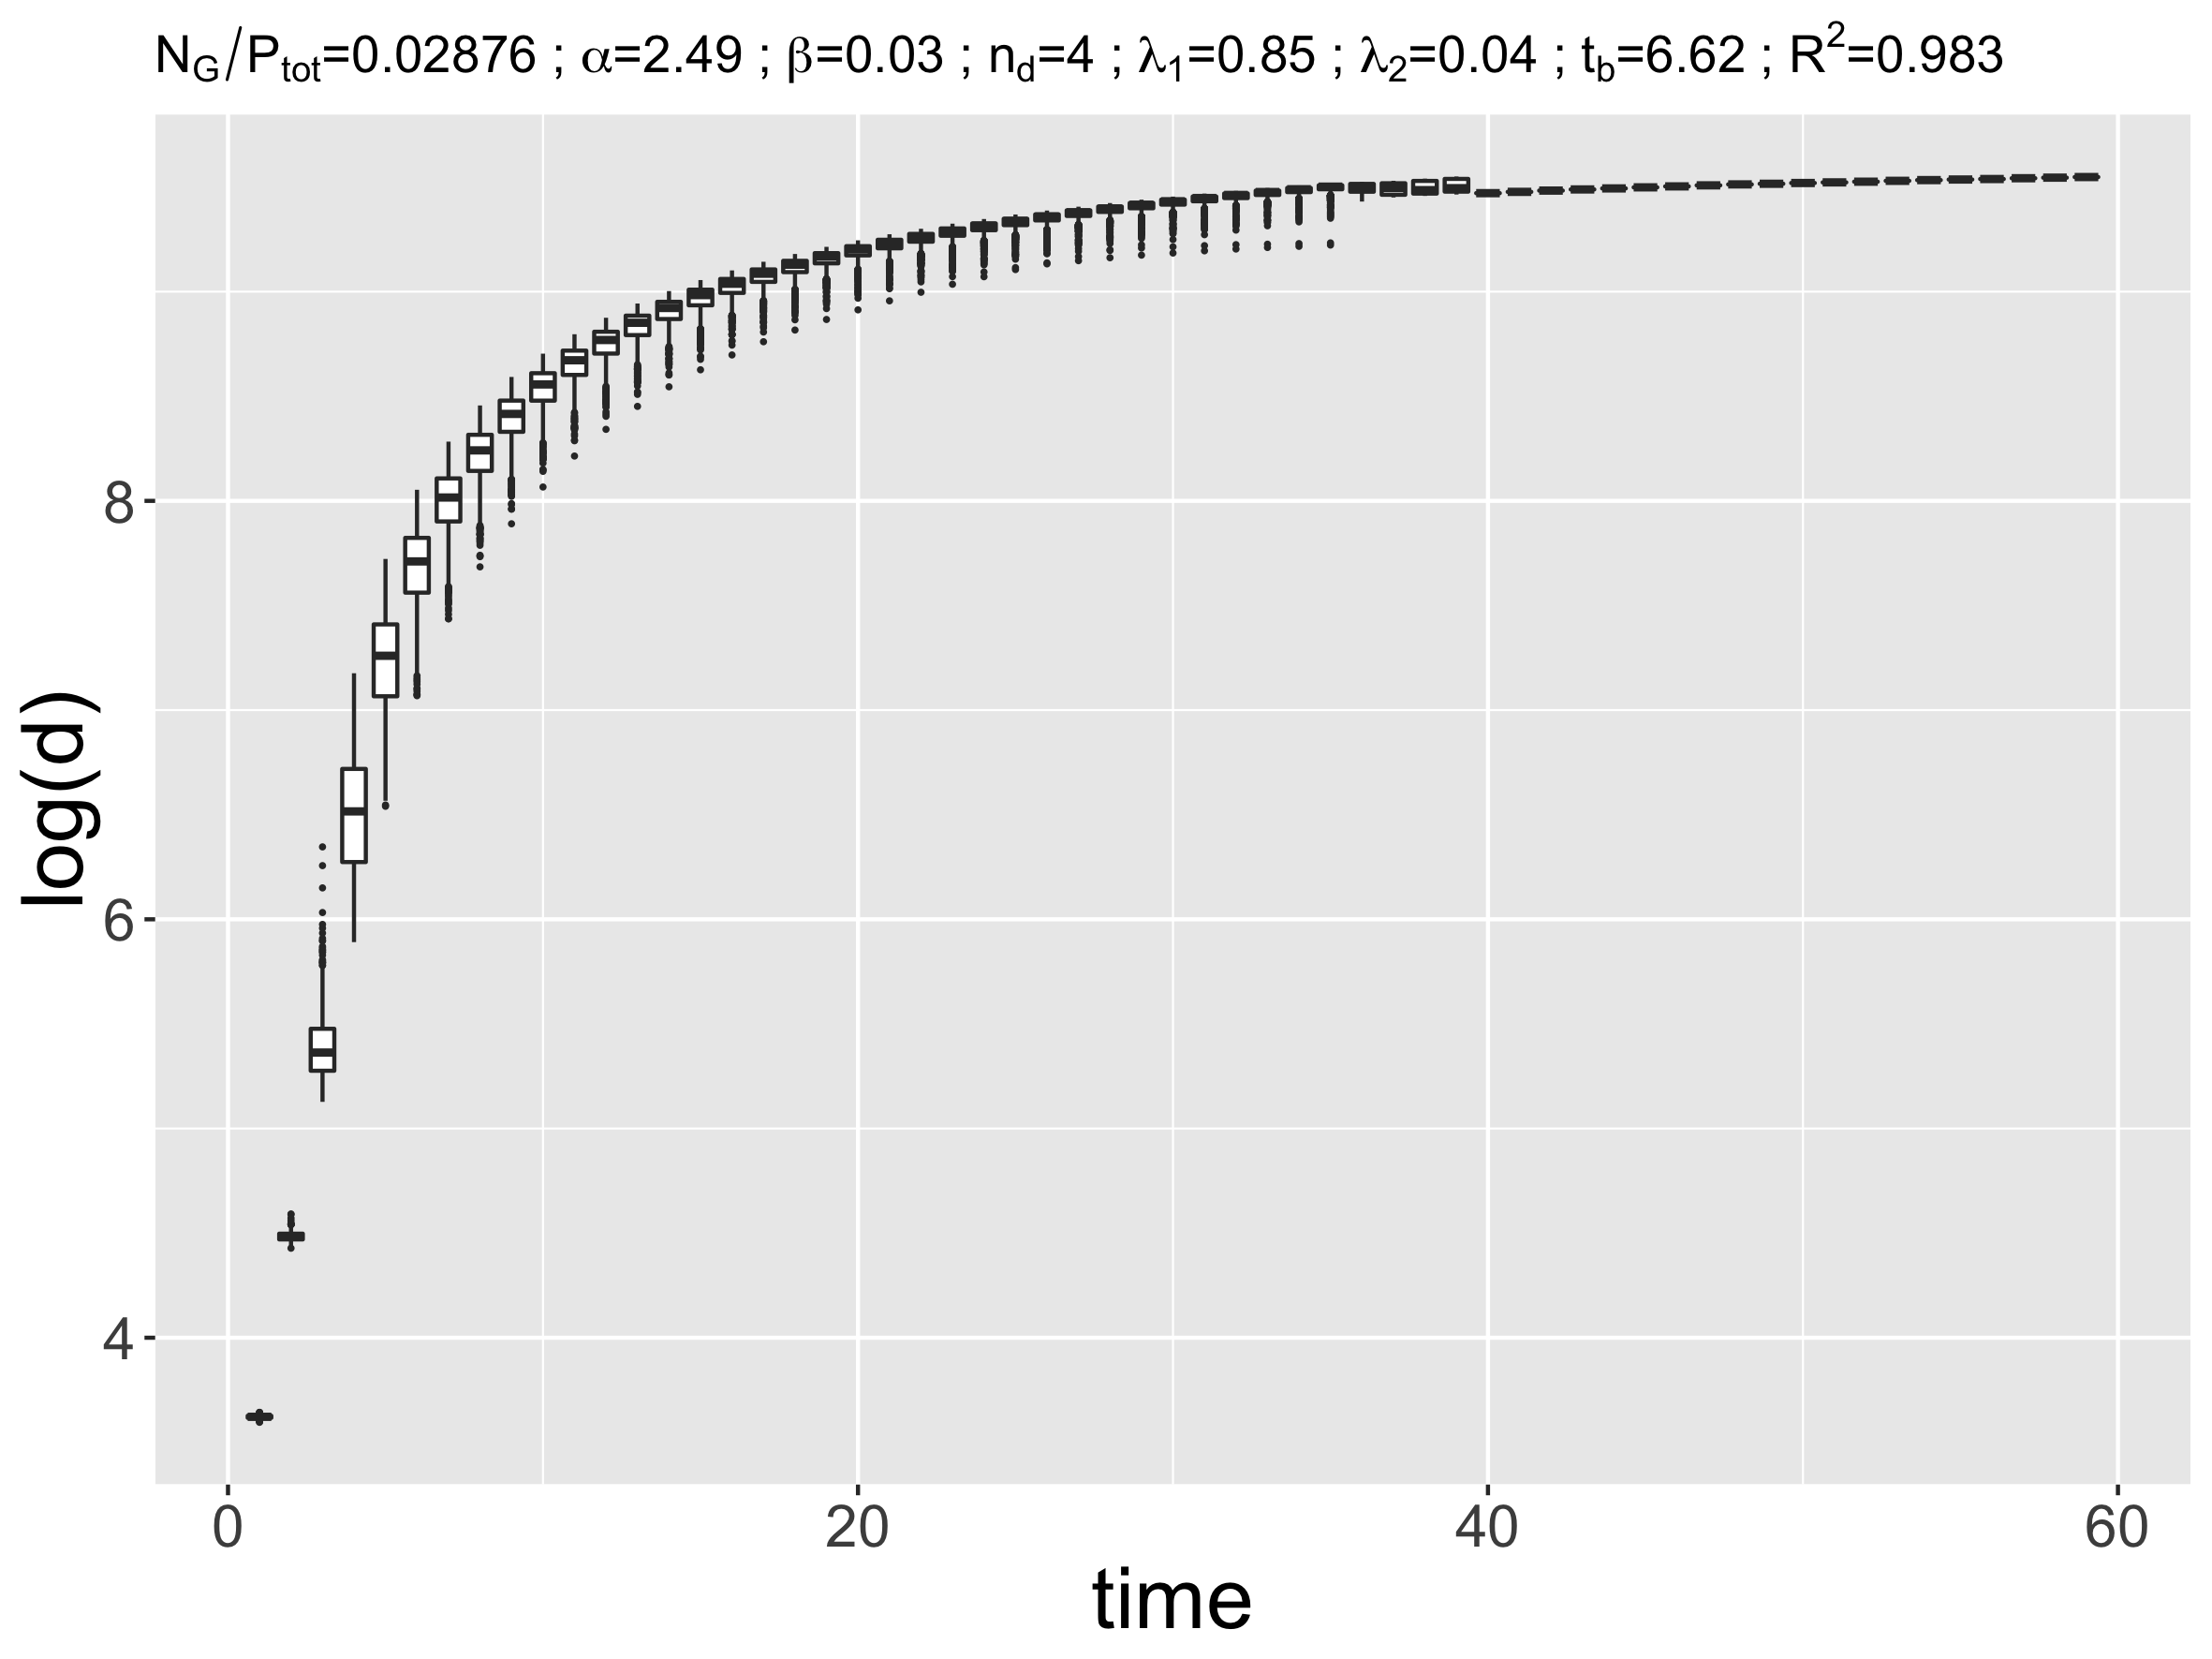
\includegraphics[width=0.49\linewidth]{figures/configdist_boxplot_id3784.png}
	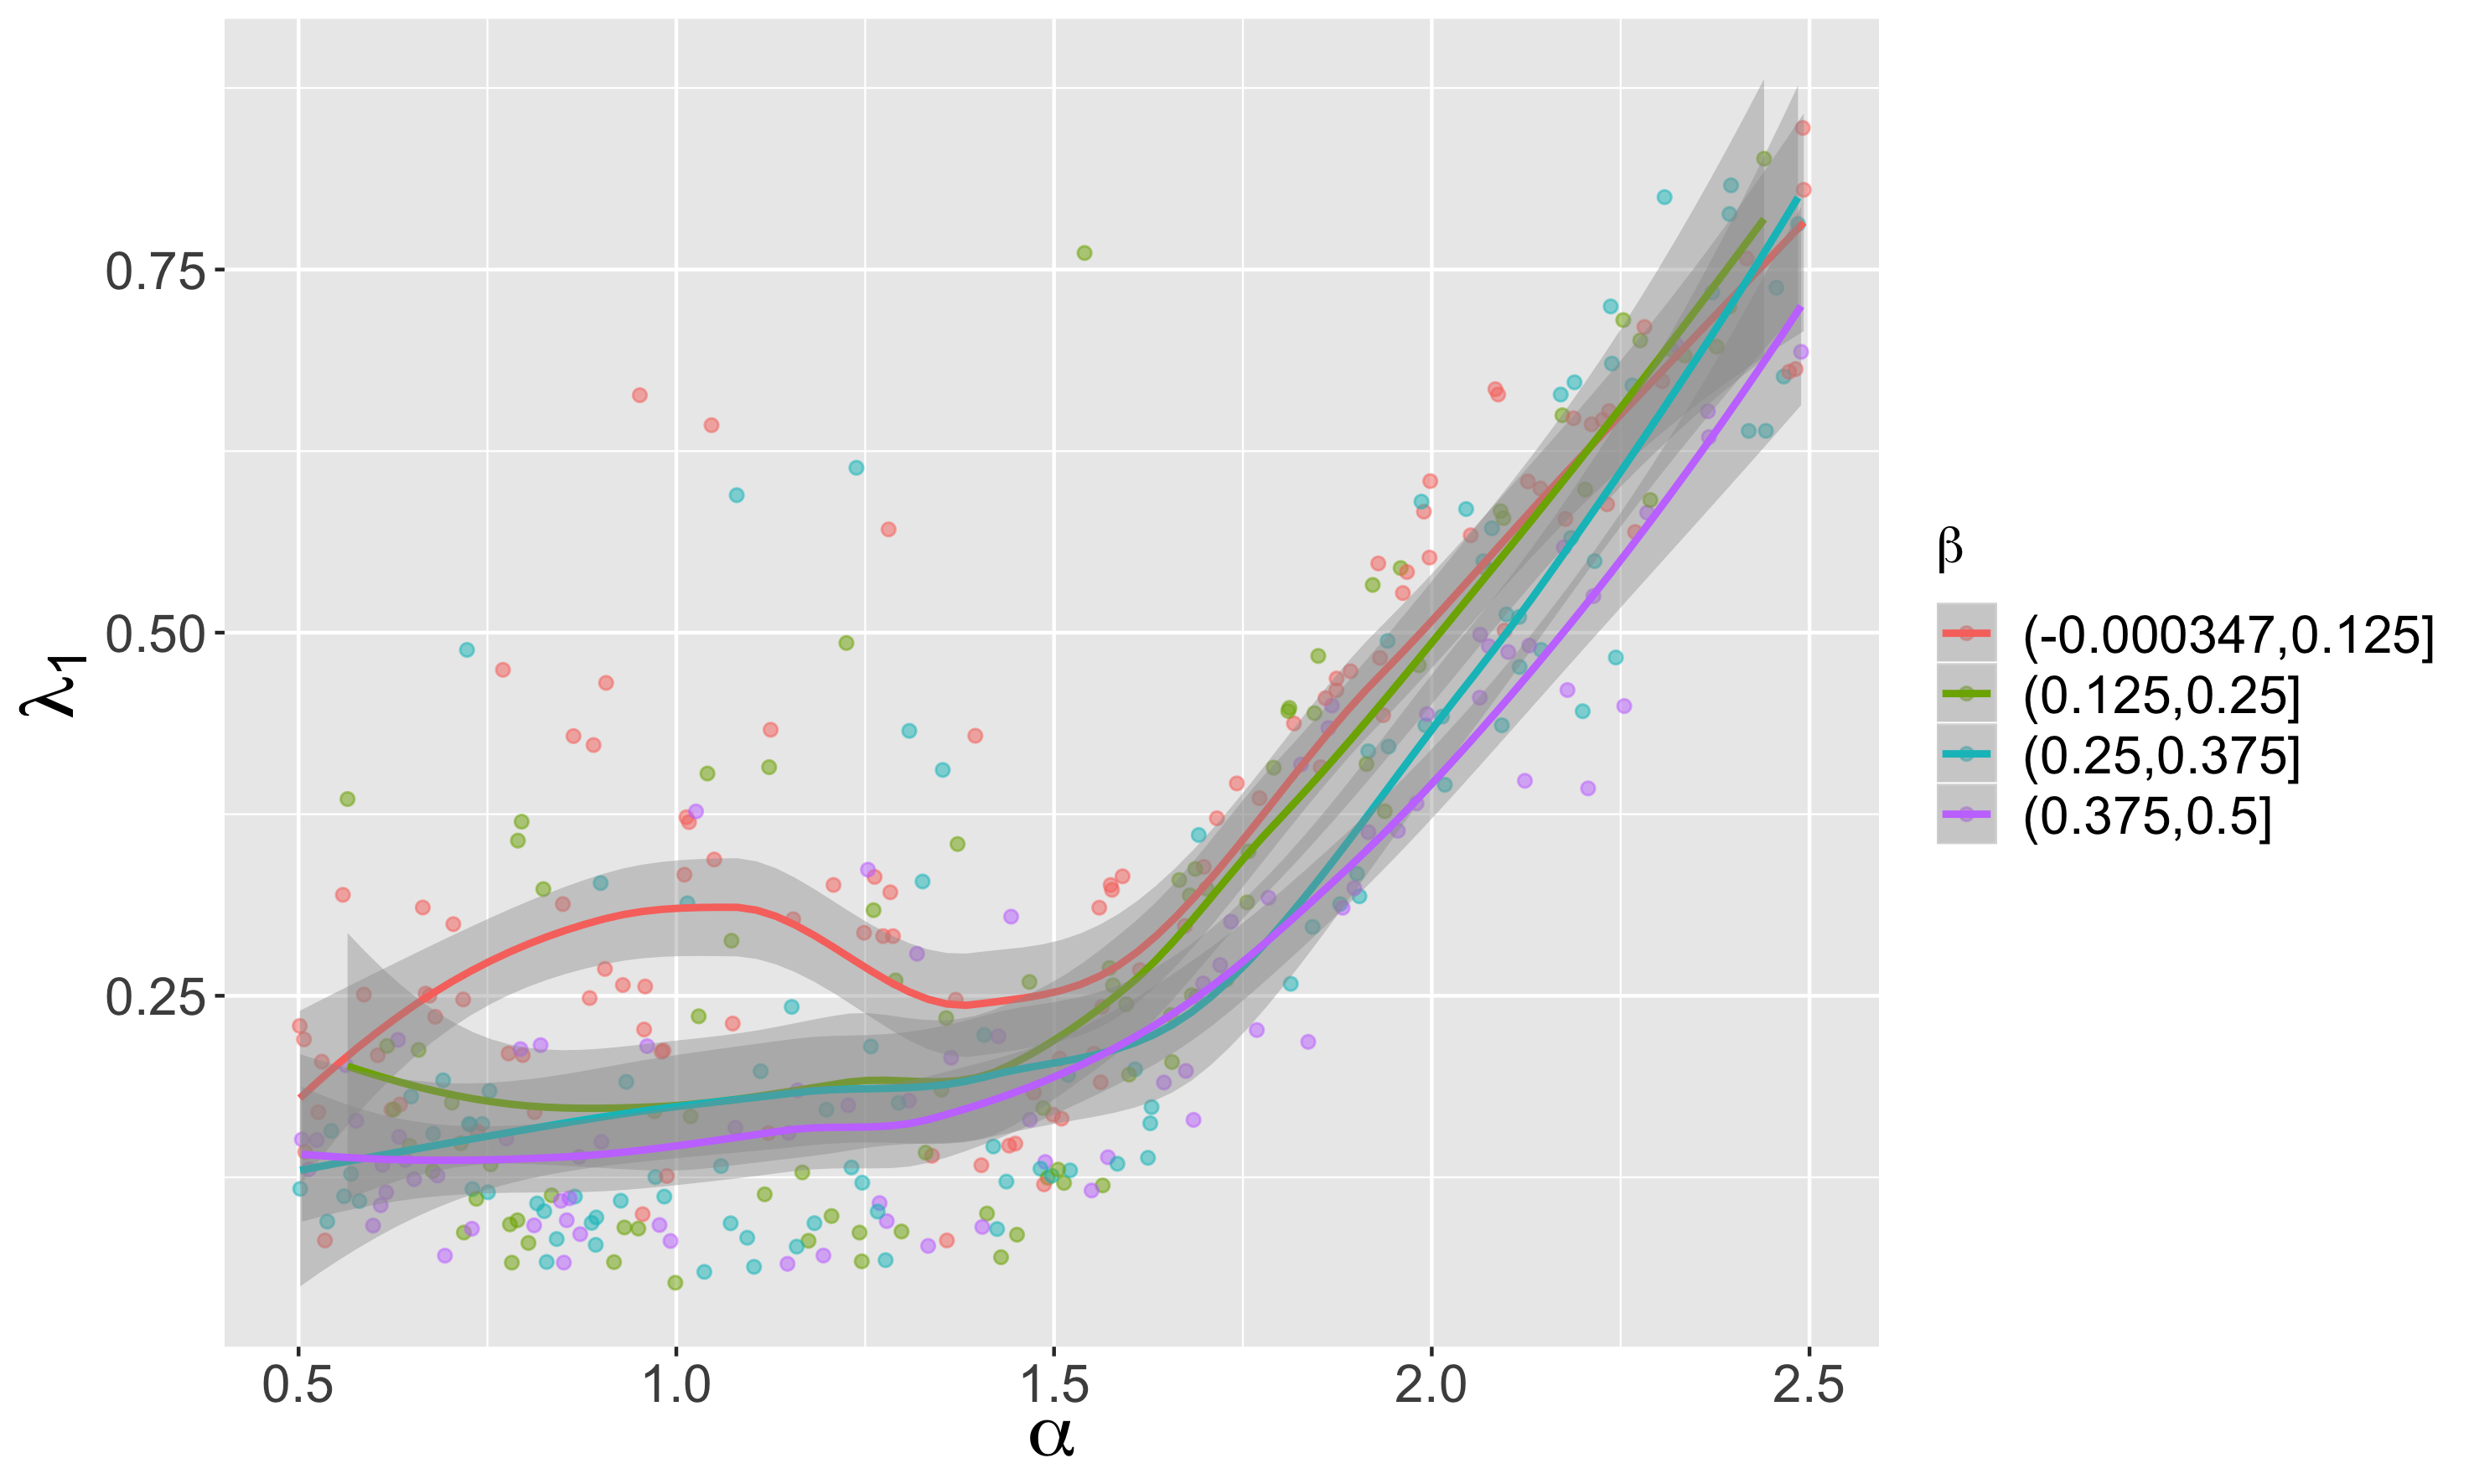
\includegraphics[width=0.49\linewidth]{figures/lambda1_alpha_colbeta.png}
	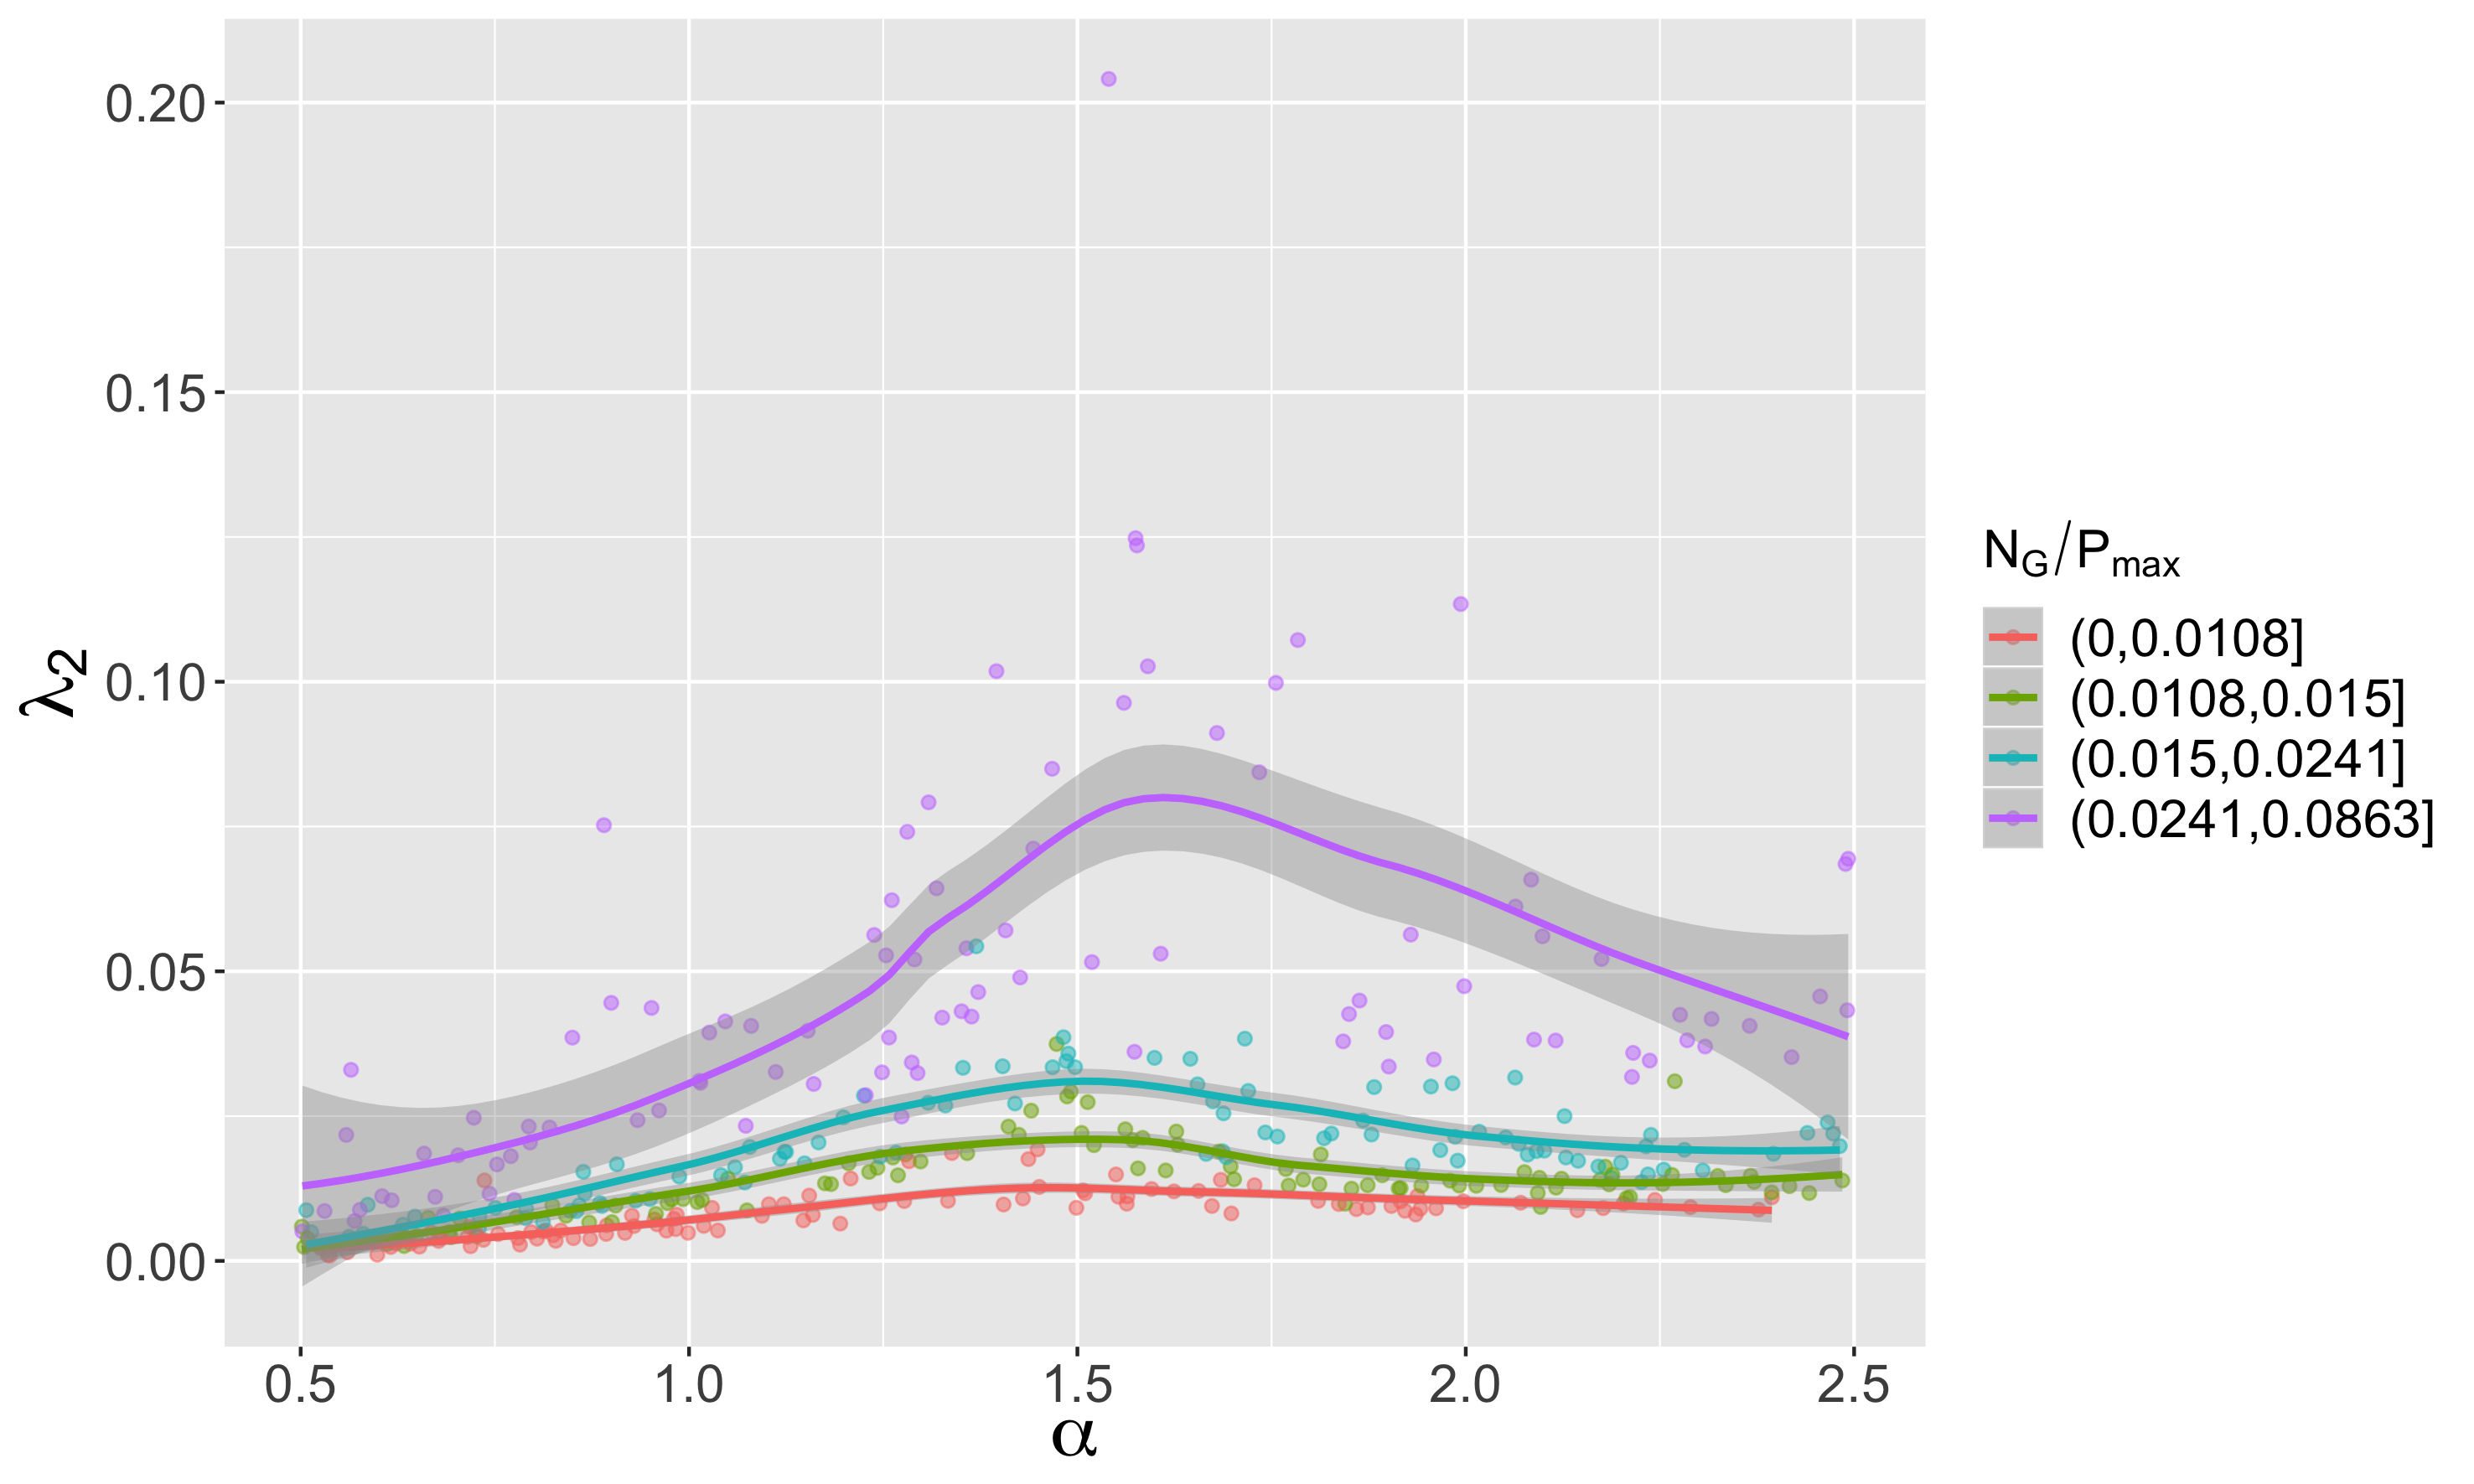
\includegraphics[width=0.49\linewidth]{figures/lambda2_alpha_colrelgrowthrate.png}
	\caption{\textbf{Estimation des exposants de Lyapounov locaux pour le modèle de Réaction-diffusion.} \textit{(Haut)} Profils temporel sous forme de statistiques descriptives pour $\log d(t)$ en fonction de $t$, pour deux configurations présentant un ajustement maximal et une valeur de $\lambda_1$ maximale ; \textit{(Bas gauche)} Valeur de $\lambda_1$ en fonction de $\alpha$, pour différentes valeurs de $\beta$ (couleur) ; \textit{(Bas droite)} Valeur de $\lambda_2$ en fonction de $\alpha$, pour différentes valeurs de $N_G / P_{max}$.}
	\label{fig:lyapounov}
\end{figure}
%%%%%%%%%%%%%

Par ailleurs, nous illustrons les trajectoires temporelles des indicateurs morphologiques agrégés. Un plan d'expérience similaire avec une seule simulation du modèle à chaque répétition et un état initial vide, mais en suivant dans le temps les valeurs des indicateurs de forme urbaine (Moran, entropie, distance moyenne, hiérarchie), montre que les trajectoires des celles-ci sont dépendantes au chemin. En effet, l'exemple de la Fig.~\ref{fig:morphotraj} montre une divergence importante des trajectoires à partir du même point initial, mais surtout des trajectoires se croisant (les indicateurs ne peuvent donc pas être formulés comme système dynamique déterministe dans lequel les trajectoires ne peuvent se croiser par le théorème de Cauchy-Lipschitz), révélant de nombreux points où la forme urbaine est très proche (au moins pour les deux indicateurs présentés) pour deux trajectoires, mais le passé et le futur sont différents. Ainsi, l'état futur d'un système urbain dépend entièrement de la trajectoire passée, et deux systèmes très similaires à un instant donné peuvent présenter des trajectoires fondamentalement différentes. Il s'agit naturellement d'une illustration par un modèle jouet, sur l'aspect particulier de la forme urbaine, mais les effets de dépendance au chemin sont a priori encore plus importants avec la prise en compte des multiples niveaux, des aspects politiques, des infrastructures \citep{pumain2012urban}.



%%%%%%%%%%%%%
\begin{figure}
	\centering
	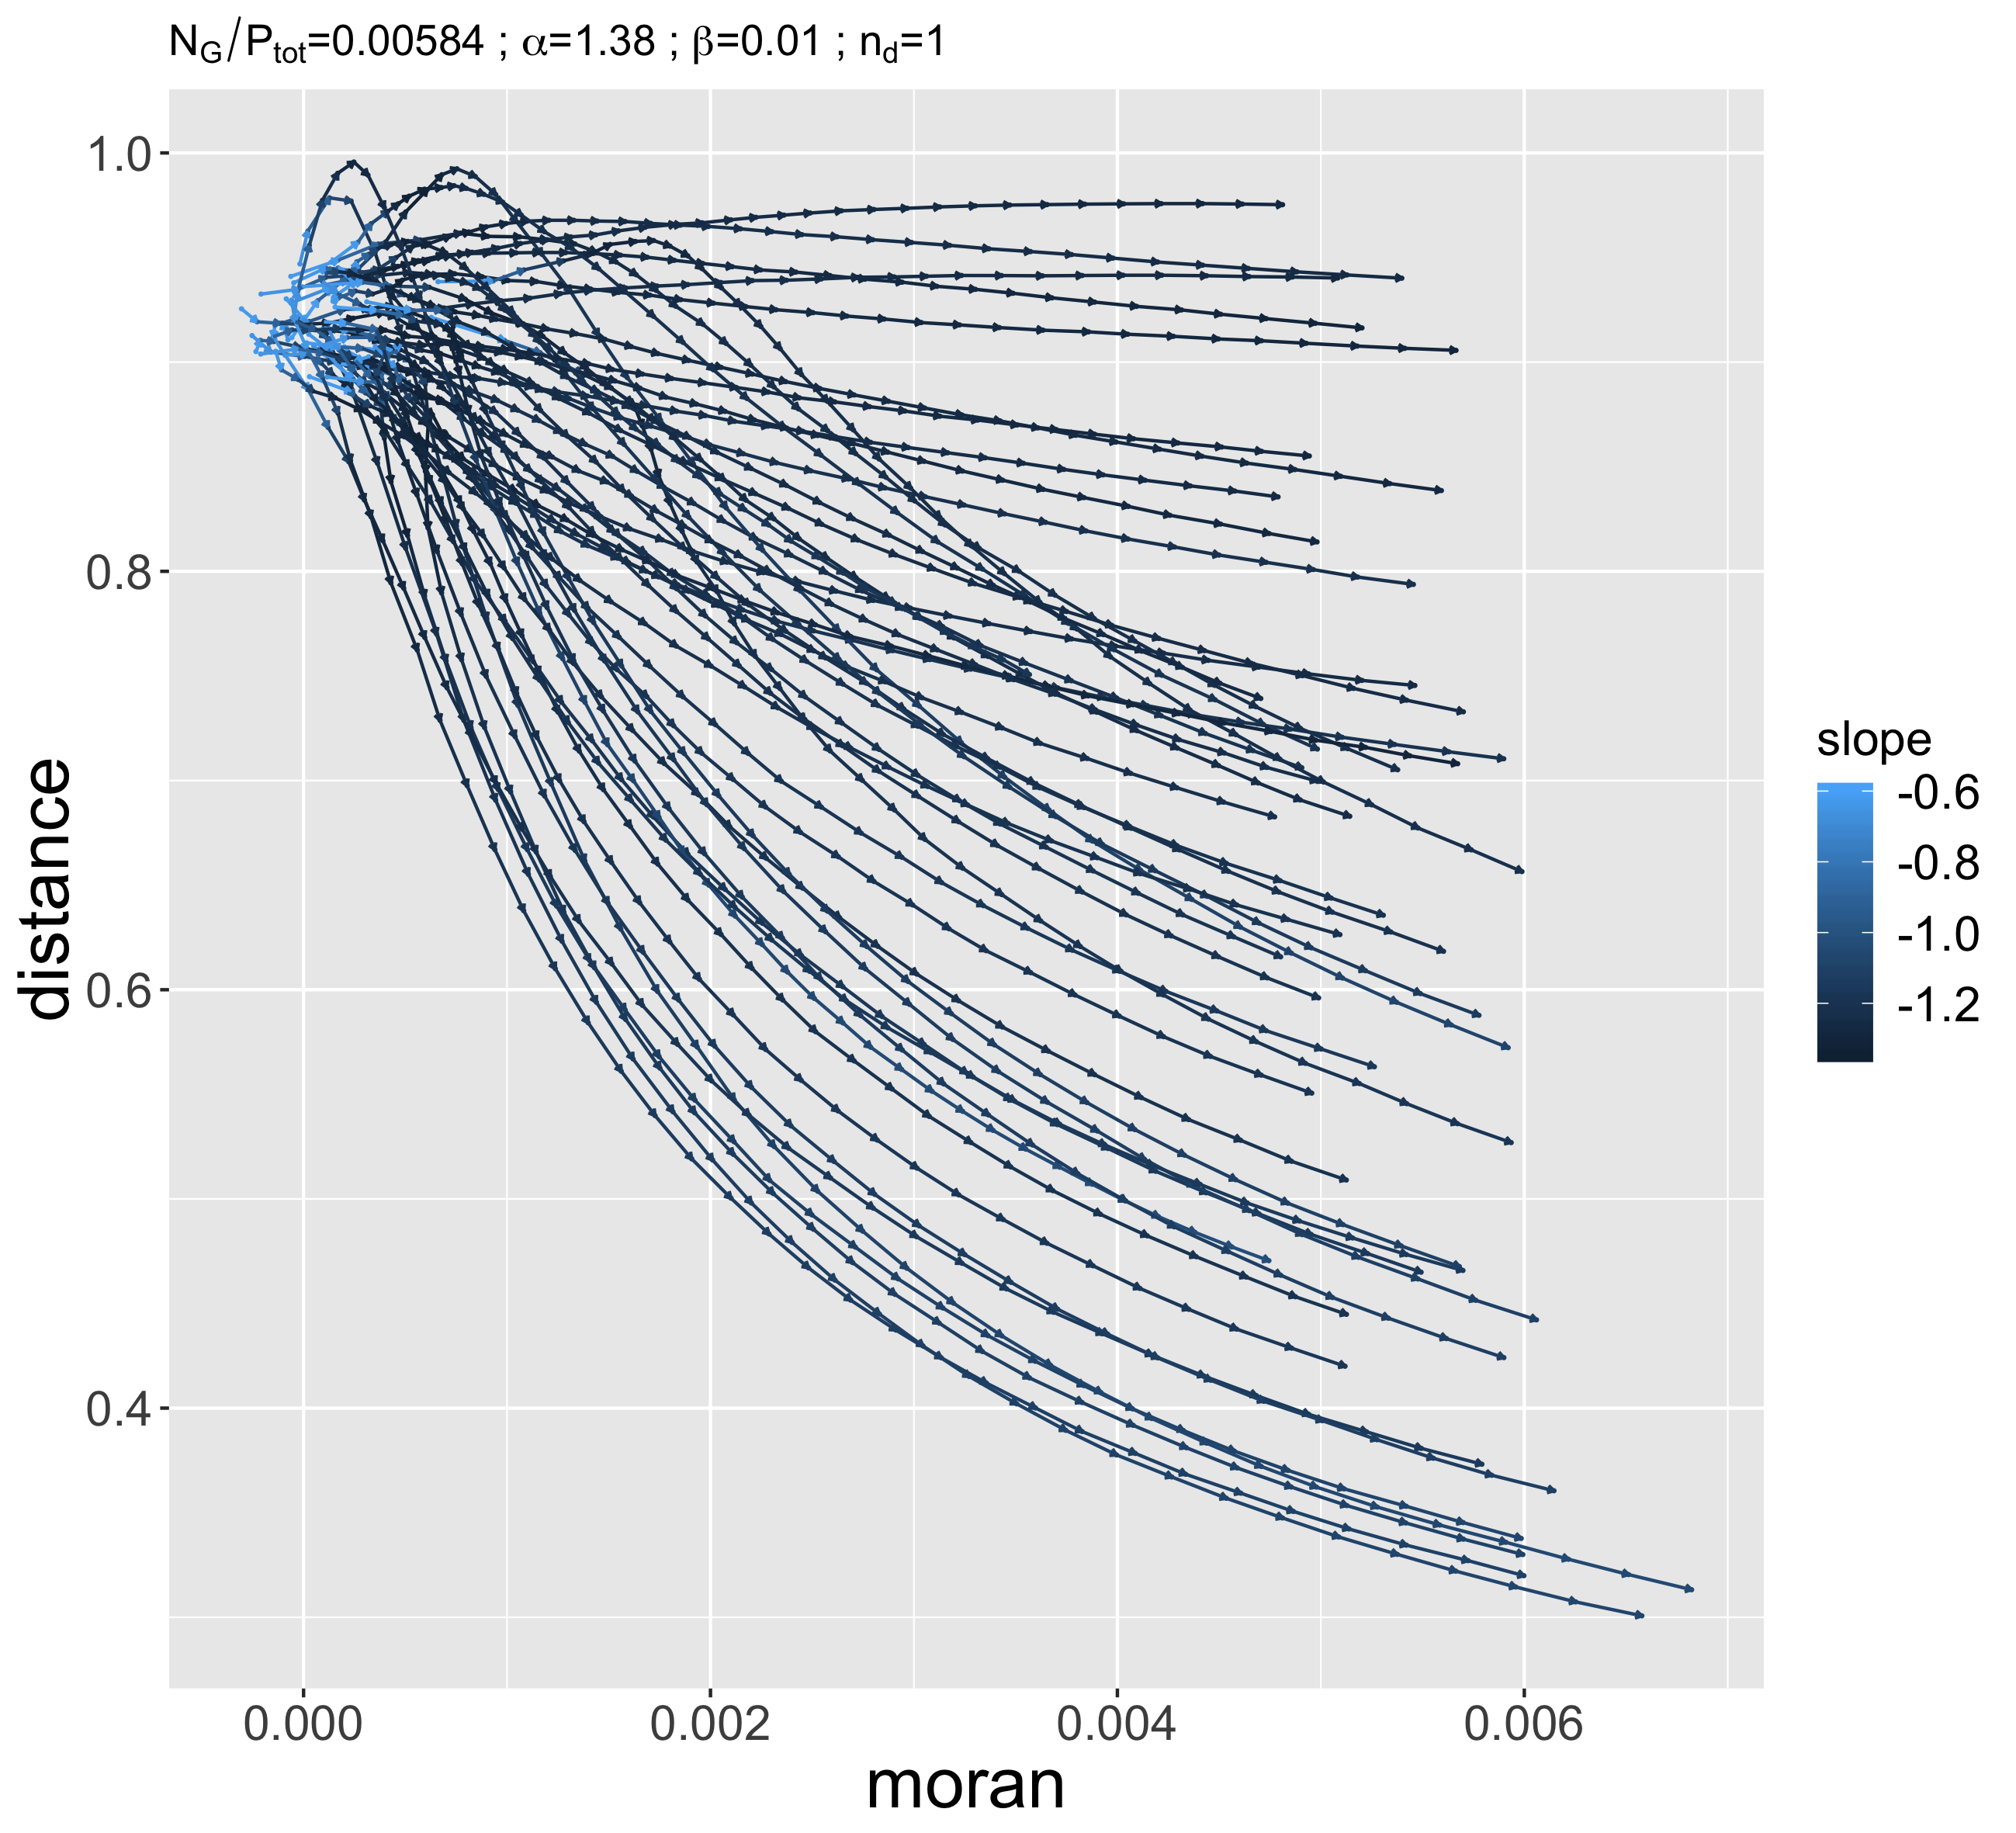
\includegraphics[width=0.7\linewidth]{figures/trajs_moran-dist_seed8578.png}
	\caption{\textbf{Trajectoires temporelles des indicateurs morphologiques.} Nous montrons pour un point de paramètre un échantillon de 50 trajectoires dans l'espace morphologique (moran,distance), la couleur donnant le niveau de hiérarchie. Dans cette configuration, la variance finale est très grande et les trajectoires sont amenées à se croiser, confirmant la dépendance au chemin pour les indicateurs morphologiques.}
	\label{fig:morphotraj}
\end{figure}
%%%%%%%%%%%%%


% quand peut-on dire non ergod ?



%%%%%%%%%%%%%%%%%
\section{Complexité et co-évolution}
%%%%%%%%%%%%%%%%%

% TODO pas chacke si effectivemebt regimes de coevol ! -> normalemdnt oui ?
% concentration des clusters vrai resultat (les regimes occurent dans des niches plus isolees)


%\subsection{Co-évolution dans les systèmes territoriaux}

Une certaine approche des systèmes complexes territoriaux privilégie le concept de co-évolution. L'intrication forte des éléments présents au sein de ce qui peut être compris comme niches territoriales, au sens des niches écologiques de \cite{holland2012signals}, est une expression d'une co-évolution et donc d'une complexité au sein de ces niches. \cite{raimbault2018modeling} montre l'émergence de ces niches spatiales au sein d'un modèle de co-évolution entre villes et réseaux de transport à l'échelle macroscopique.

%\subsection{Non-stationnarité spatiale et co-évolution}

Nous explorons alors ici par des expériences de simulation le lien entre non-stationnarité spatiale, qui est également un marqueur de complexité spatiale, et émergence de niches au sein d'un modèle de morphogenèse hybride couplant développement urbain et réseau, introduit par~\cite{raimbault2014hybrid}.

Le modèle RBD~\citep{raimbault2014hybrid} couple de manière simple croissance urbaine et évolution du réseau viaire. La flexibilité des régimes qu'il permet de capturer fournit dans~\cite{raimbault2017identification} un test pour une méthode d'identification de causalités spatio-temporelles. Nous étendons ici cette méthode par une détection endogène des zones spatiales correspondant à différents régimes, afin de montrer l'émergence de niches par la non-stationnarité. Pour une description précise du modèle ainsi que son utilisation comme producteur de données synthétiques, se référer à \cite{raimbault2018caracterisation}. Dans notre cas, les paramètres variables sont le nombre de centres initiaux $N_C$ ainsi que les poids relatifs des différentes variables explicatives $(w_c,w_r,w_d)$ (distance au centre, distance au réseau, densité) régissant la valeur locale lors de l'étalement urbain.

% Experimental setup:
%  - fixed distrib of field centers weight values ; repetitions with varying positions.
%  -> indicators : optimal number of niches ? "modularity" of these ? [idea : construct neighborhood network, weight = correlation, then modularity detection ?)

La non-stationnarité est introduite en faisant ces derniers paramètres de poids varier dans l'espace. Nous distinguons deux implémentations, étant donné des valeurs attribuées à chaque centre : (i) la valeur locale des poids est donnée par celle du centre le plus proche ; (ii) la valeur locale est la moyenne des valeurs des centres pondérée par les distances à ceux-ci.

Les niches spatiales sont détectées par classification non-supervisée sur les profils de corrélation retardées estimées localement dans l'espace, c'est-à-dire $(\rho_{\tau}\left[X_i,X_j\right])_{\tau,i,j}$ où $- \tau_M \leq \tau \leq  \tau_M$ avec $\tau_M = 5$, pour les trois couples de variables tels que $i < j$. Les séries temporelles sont tronquées au dessous de $t_0 = 5$ et à un point spatial donné, les corrélations sont estimées sur les cellules dans un rayon de $r_0 = 10$, avec un pas spatial de $\delta x = 5$ entre les points d'estimation. Un algorithme des k-means est utilisé pour classifier les profils, avec un nombre de clusters $k = N_C$. Pour supprimer la stochasticité de la classification, celle-ci est répétée $b = 1000$ fois, et les mesures de performance sont estimées sur l'ensemble de ces réalisations de la classification.

%Distance entre partitions \cite{porumbel2011efficient} \cite{day1981complexity} \cite{gusfield2002partition} \cite{rossi2011partition}
Afin de quantifier la classification, une solution pourrait être d'étudier une distance à la partition définie par les zones de stationnarité. Cependant, la détermination d'une distance entre partitions est un problème NP-difficile \citep{day1981complexity} dont même les solutions optimales \citep{porumbel2011efficient} dépassent les capacités de calcul vu le nombre de réalisations. Nous utilisons donc les indicateurs suivants, capturant des propriétés attendues de niches spatiales : (i) distance cumulée entre les centroïdes de la classification et les centres, corrigée par la distance entre les centroïdes et celle entre les centres % formule ?
 ; (ii) rayon normalisé moyen des clusters ; (iii) distance moyenne entre les vecteurs de features utilisés pour la classification ; (iv) variance intra-cluster moyenne. Chaque indicateur est calculé sur la classification obtenue ainsi que sur un modèle nul donné par une redistribution aléatoire des étiquettes de cluster entre les points.
 
 
%%%%%%%%%%%%%%
\begin{figure}
	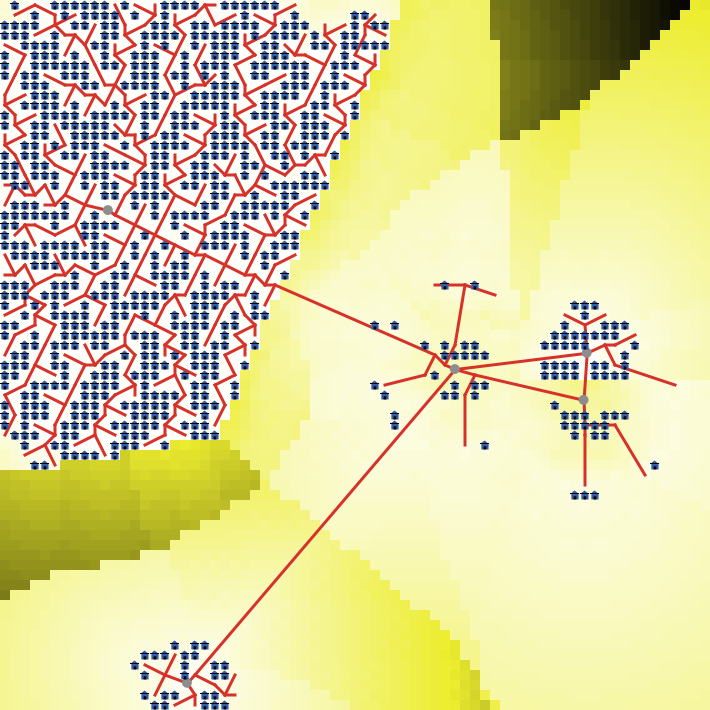
\includegraphics[width=0.49\textwidth]{figures/ex_0_tf30.png}
	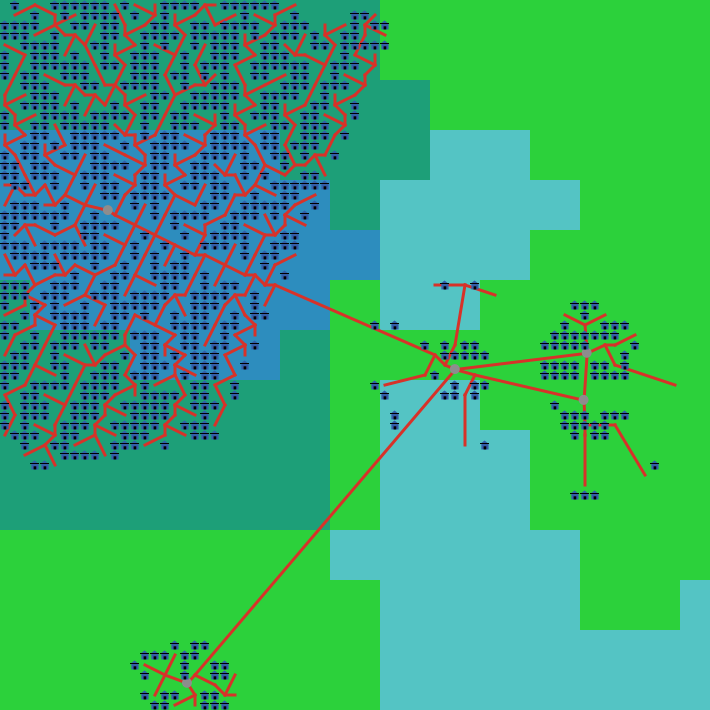
\includegraphics[width=0.49\textwidth]{figures/ex_0_tf30_rsclustering321.png}\\\bigskip
	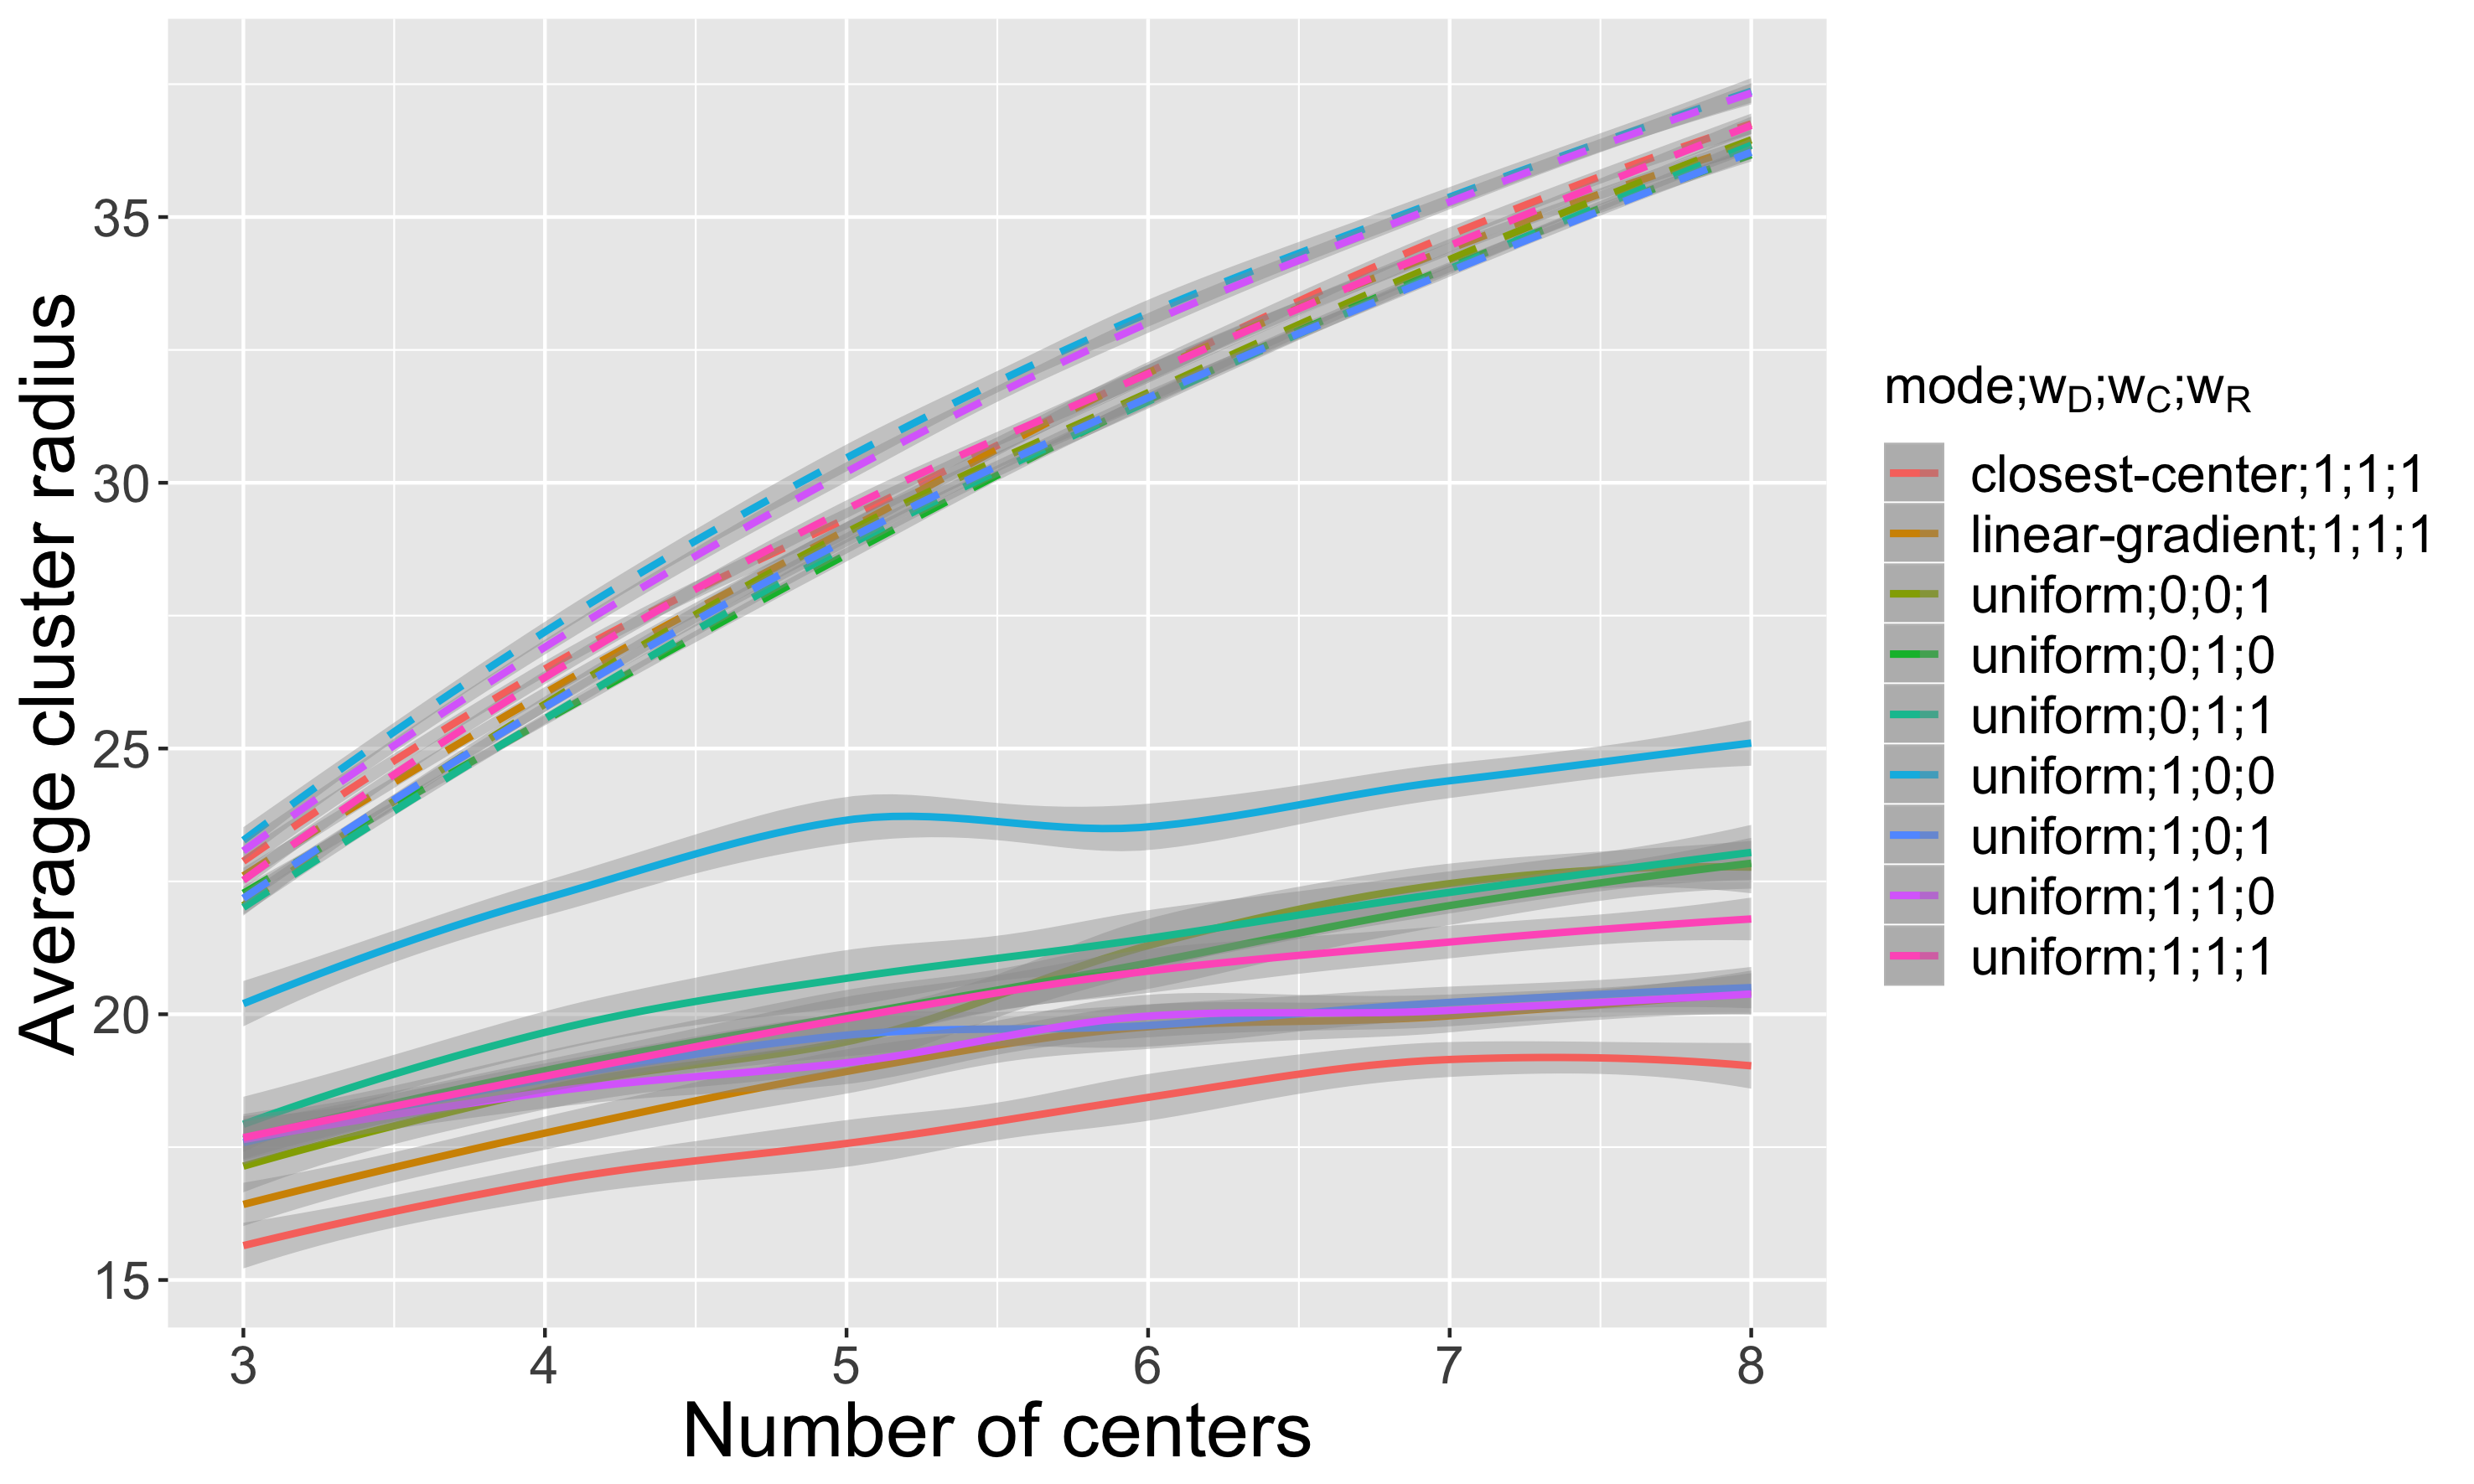
\includegraphics[width=0.49\textwidth]{figures/radius.png}
	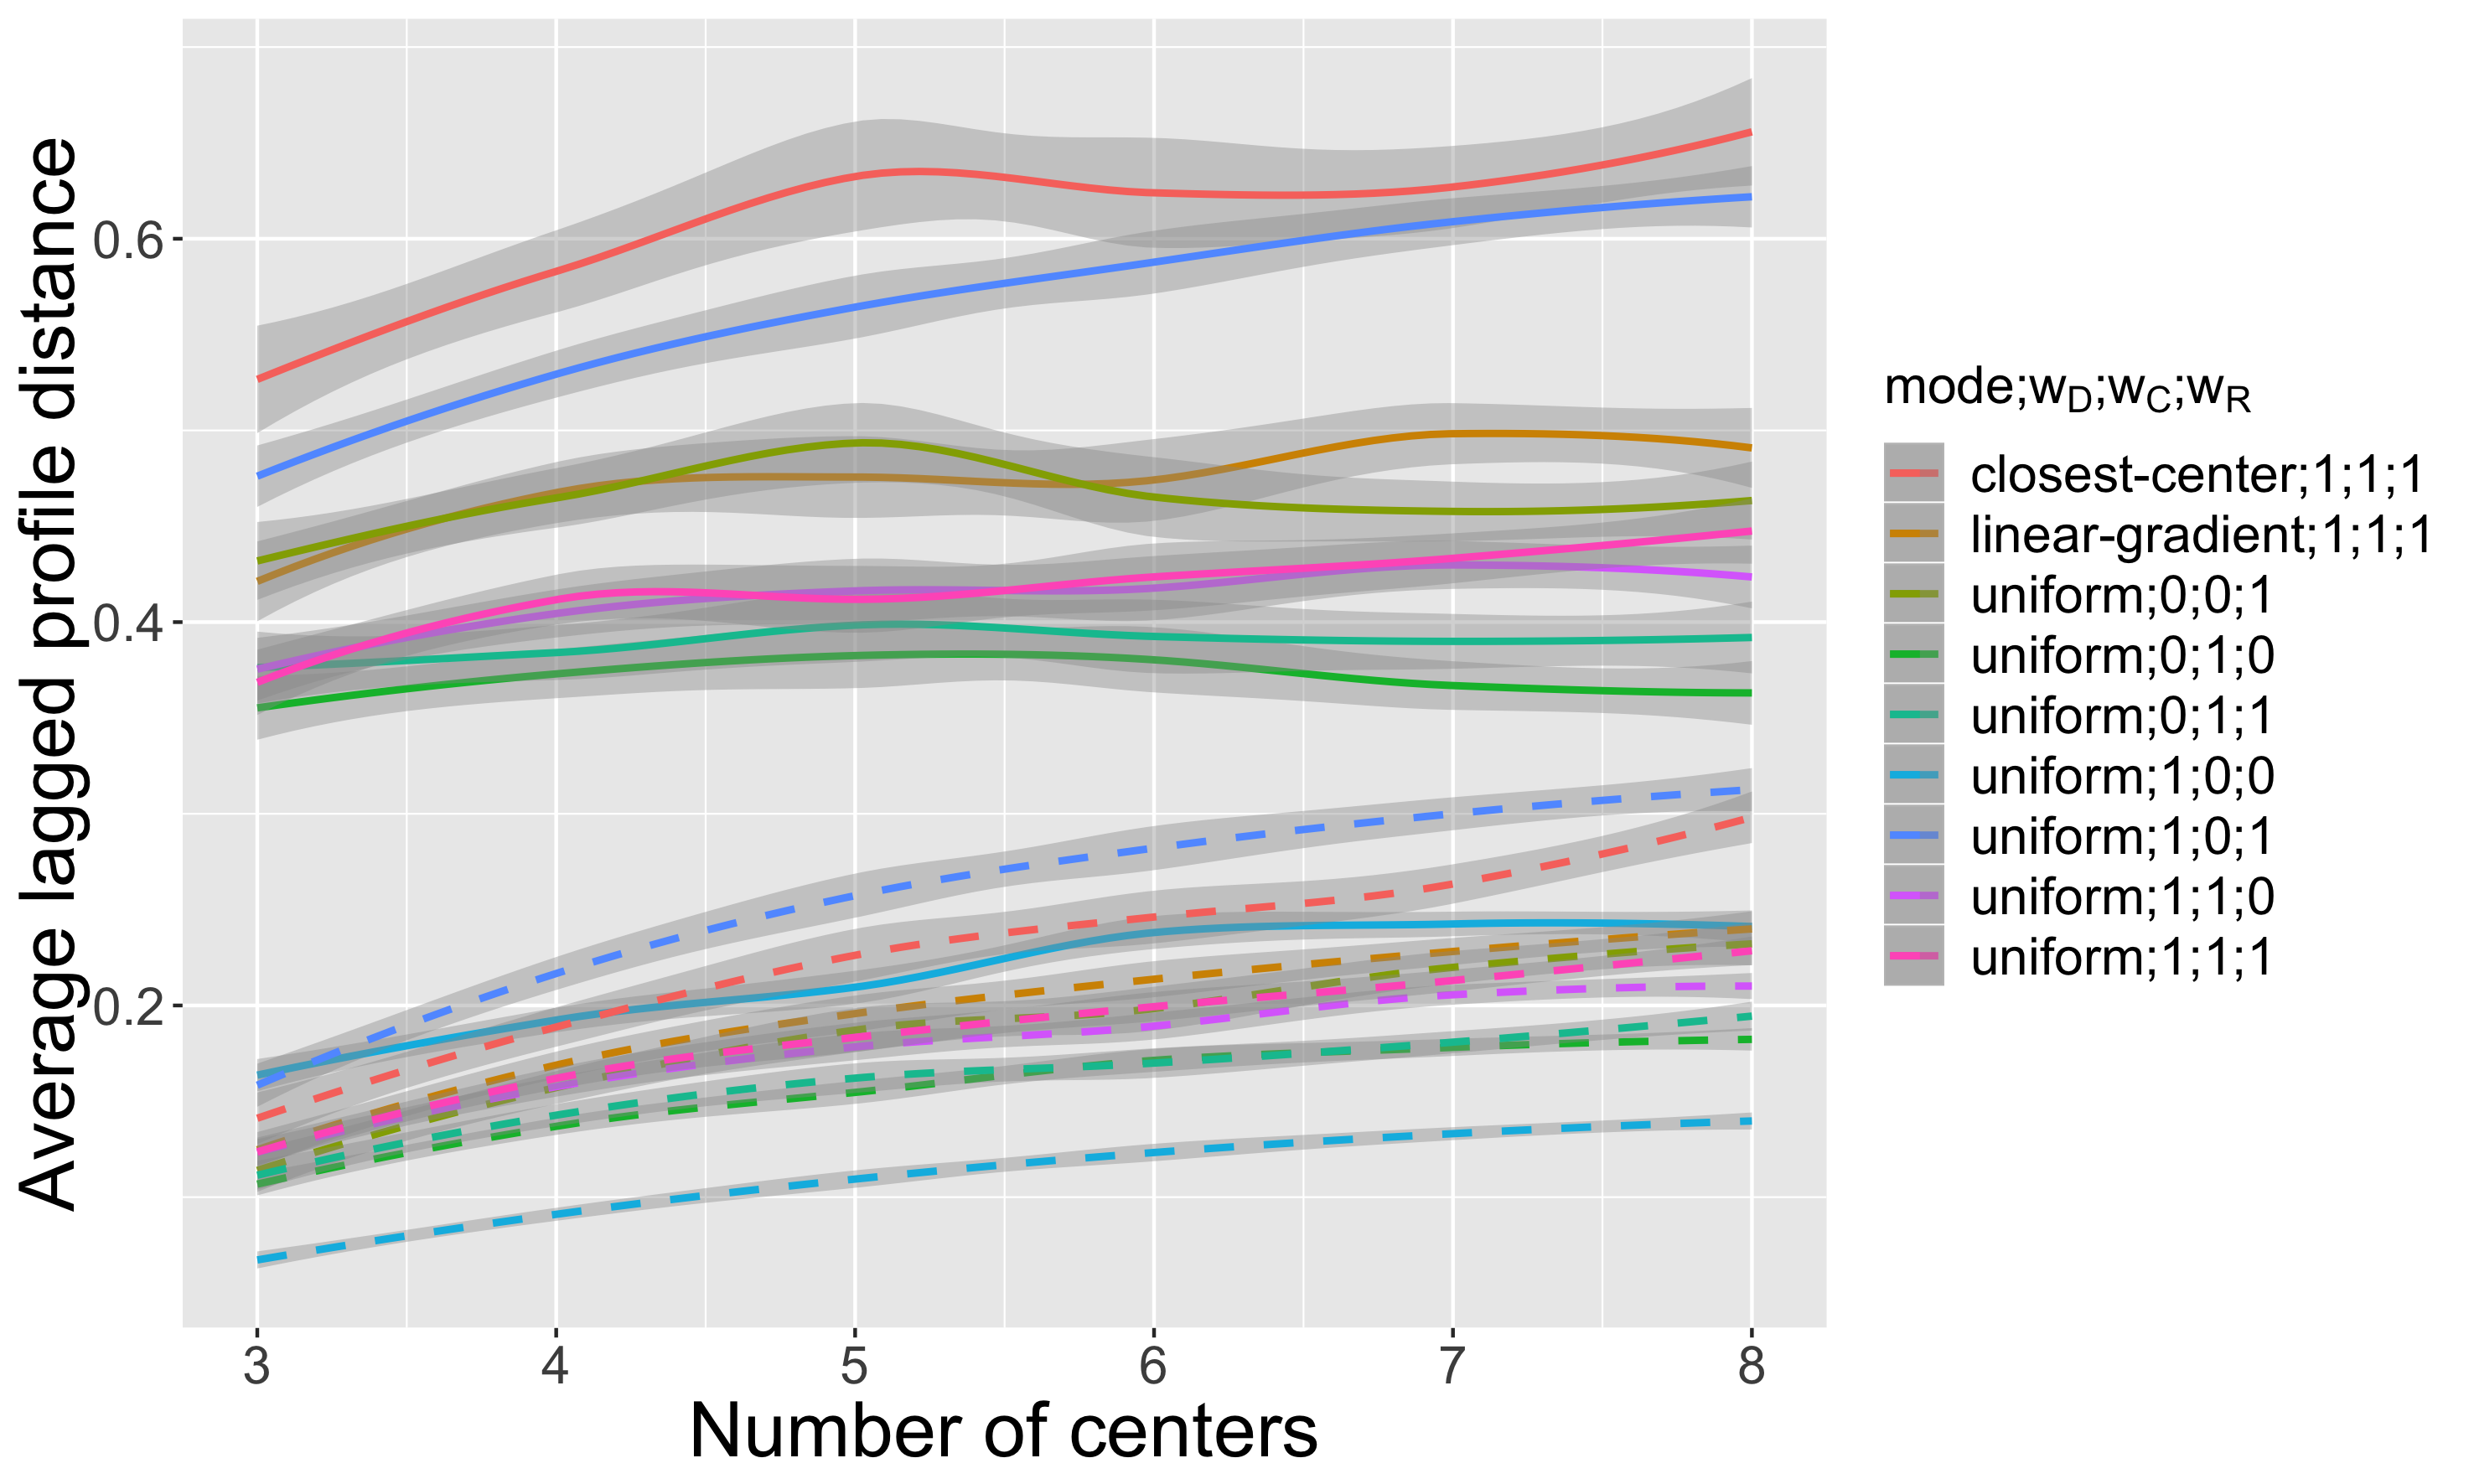
\includegraphics[width=0.49\textwidth]{figures/profiledisteucl.png}\\
	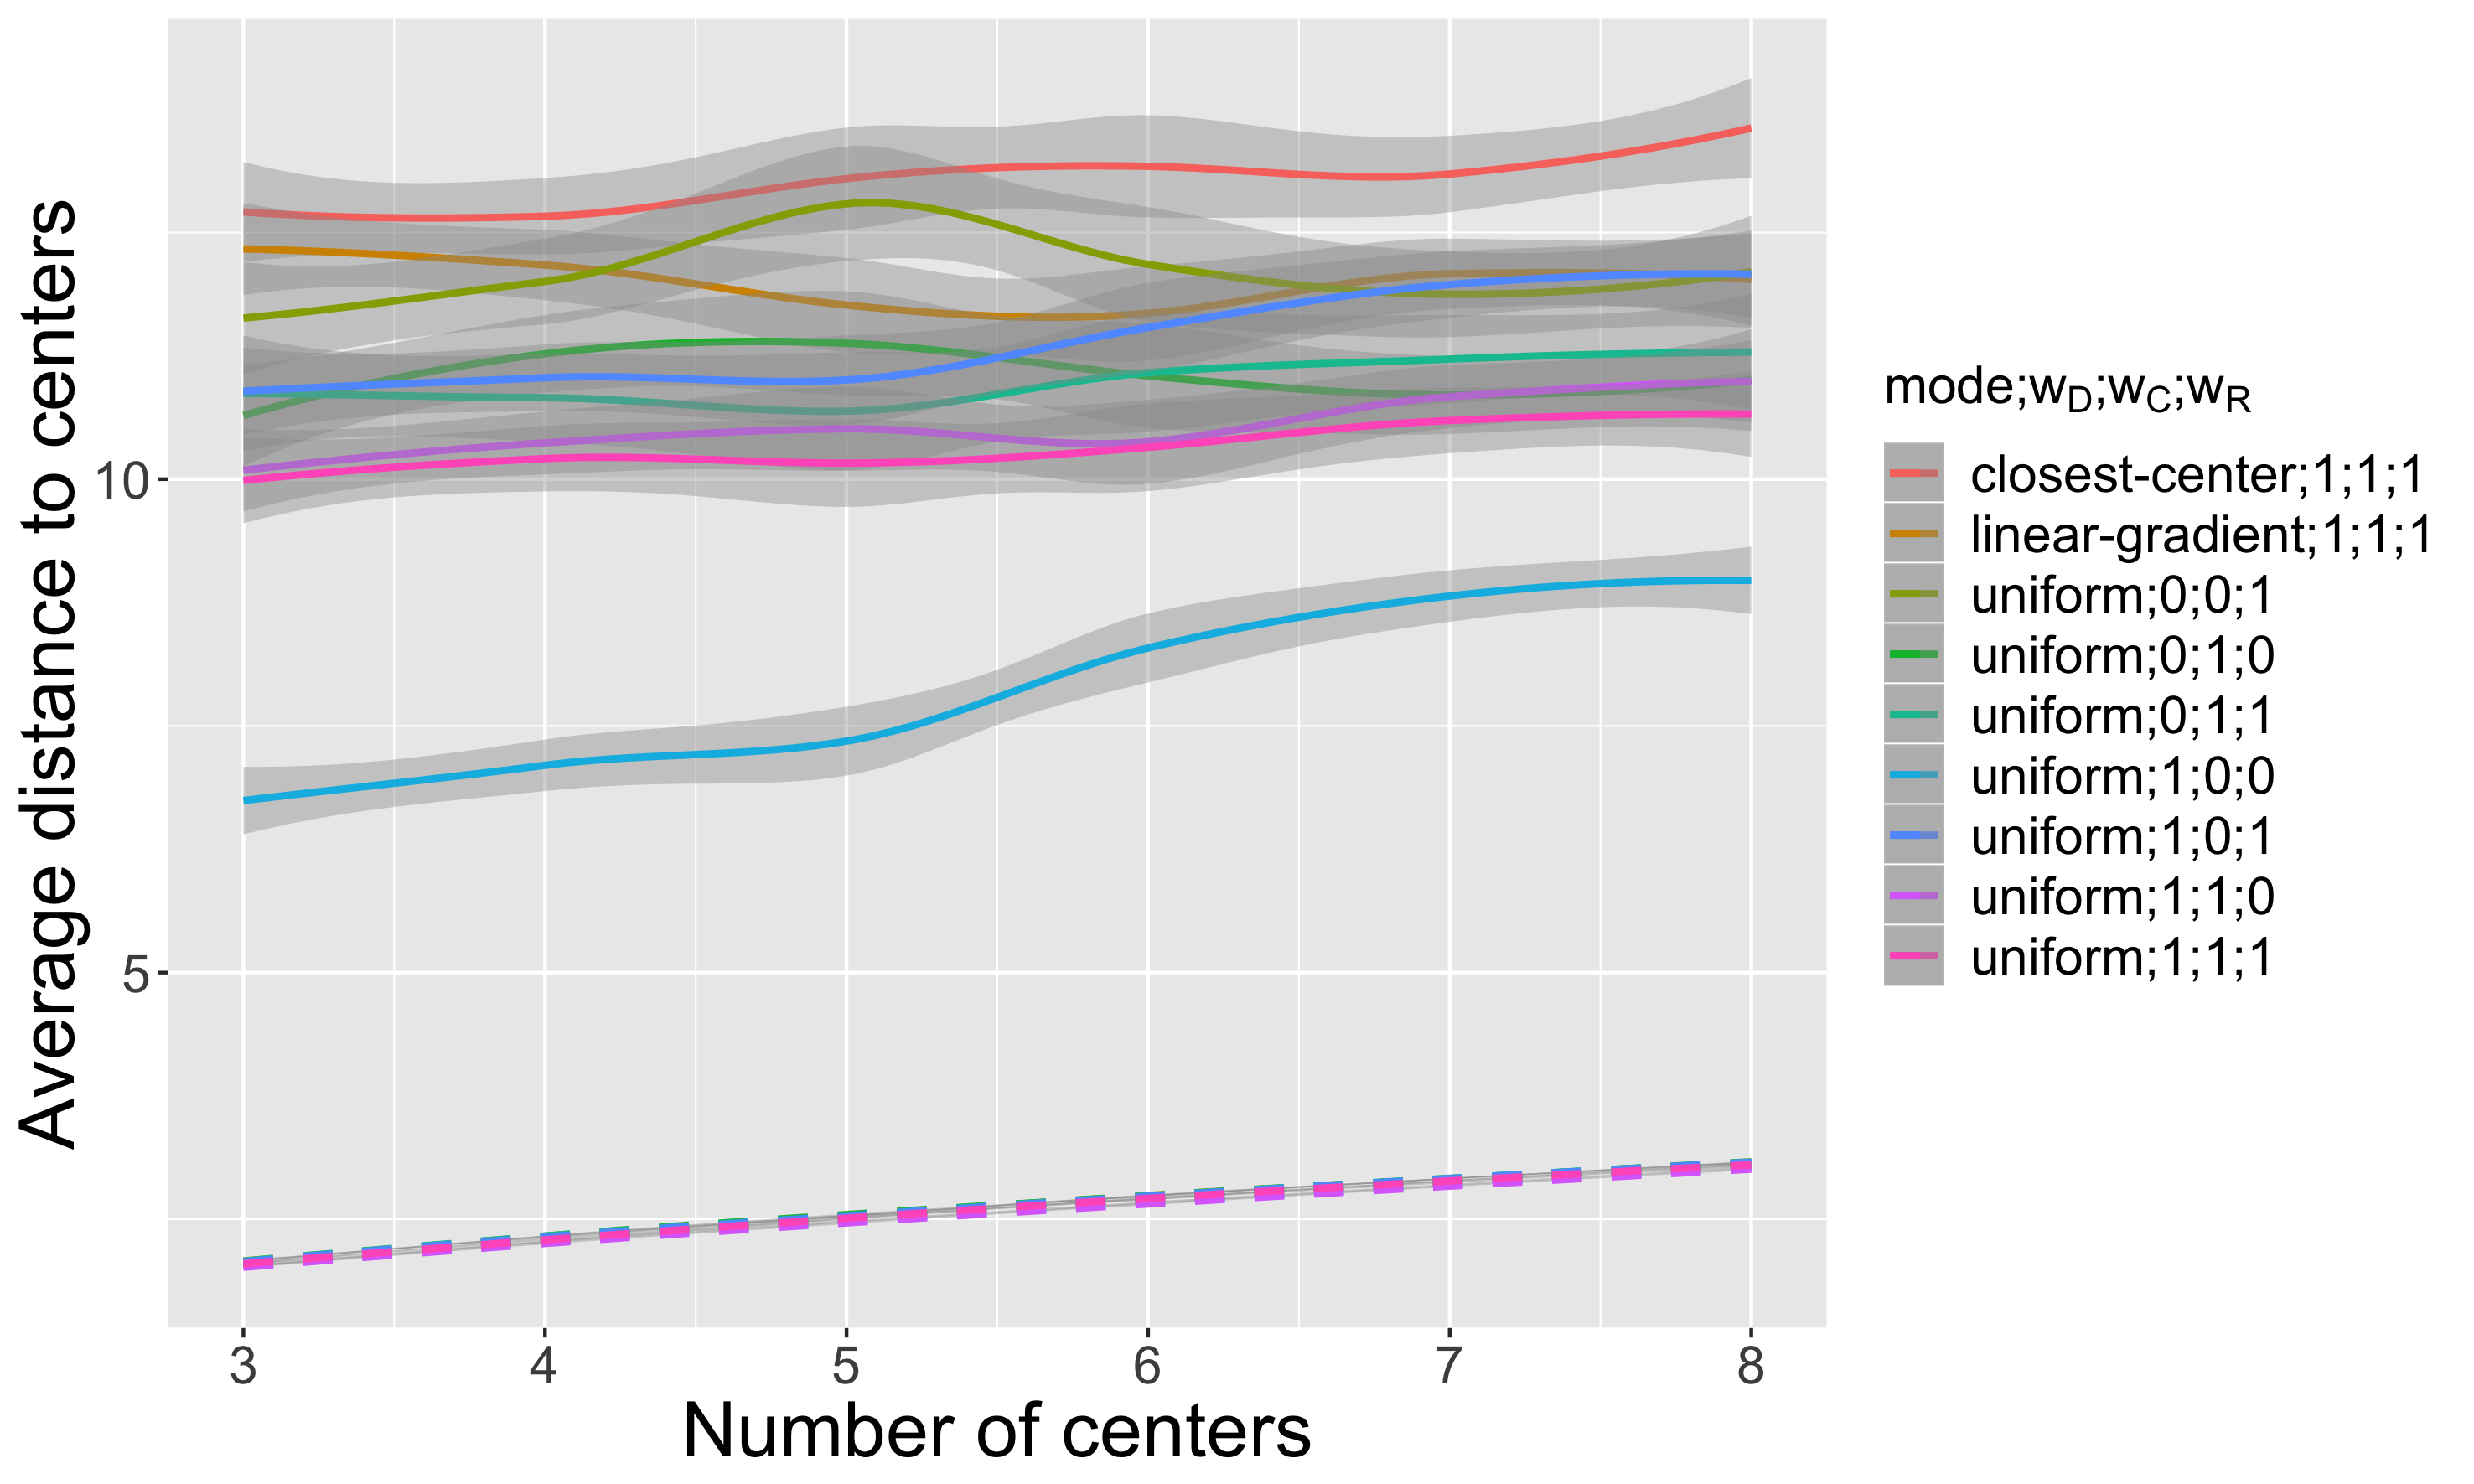
\includegraphics[width=0.49\textwidth]{figures/distance.png}
	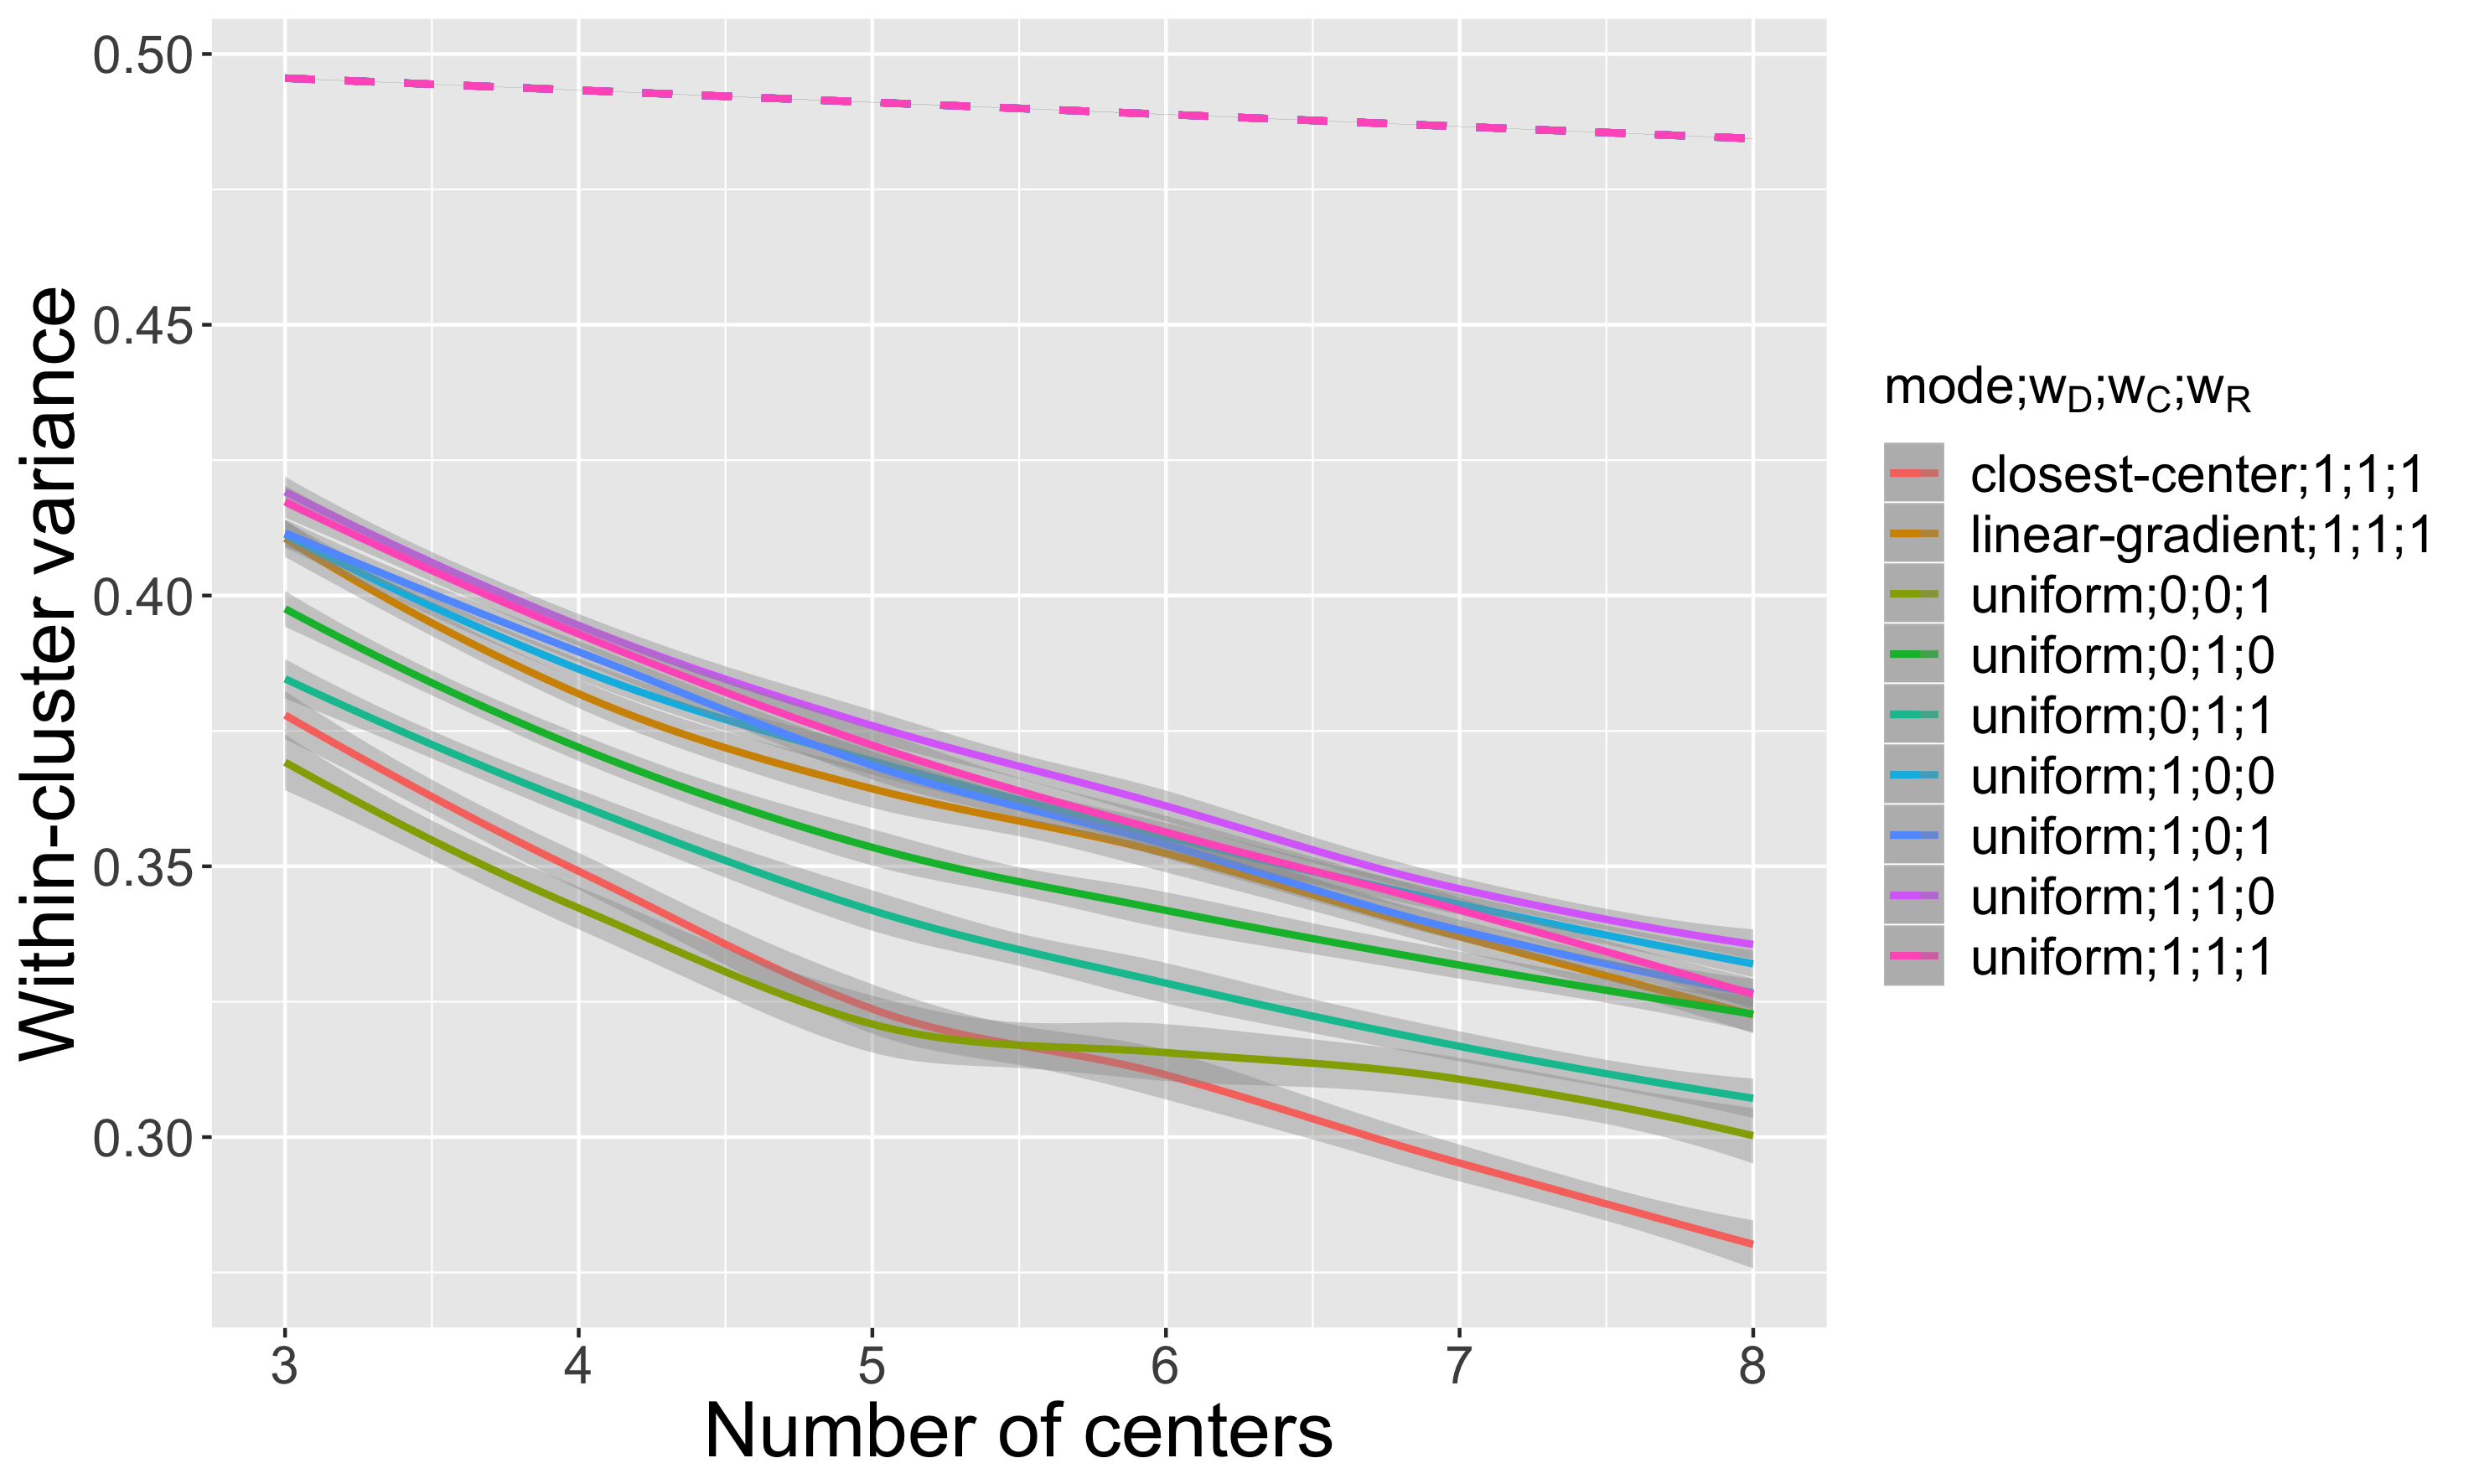
\includegraphics[width=0.49\textwidth]{figures/withinss.png}
	\caption{\textbf{Niches spatiales de co-évolution dans le modèle RBD.}\textit{(Haut gauche)} Configuration générée avec $N_C = 5$ centres et des paramètres non-stationnaires par centre le plus proche, tels que, dans un ordre de coordonnée verticale décroissante, les poids pour chaque centre sont $(w_d,w_r,w_c) = (0,1,0) ; (0,0,1) ; (1,0,1) ; (1,0,1) ; (0,0,1)$ ; \textit{(Haut droite)} Exemple de réalisation correspondante pour la classification par k-means, la couleur de cellule donnant le cluster ; \textit{(Milieu gauche)} Rayon normalisé moyen des clusters, pour chaque mode et configuration de paramètres (couleur), ainsi que pour le modèle nul de cluster aléatoire (lignes pointillées) ; \textit{(Milieu droit)} Distance moyenne entre les profils de corrélations retardées pour les centroïdes des clusters ; \textit{(Bas gauche)} Distance moyenne des centroïdes aux centres ; \textit{(Bas droite)} Variance intra-cluster.}
	\label{fig:rbd}
\end{figure}
%%%%%%%%%%%%%%

 
 
Notre plan d'expérience compare les deux modalités de non-stationnarité (distributions aléatoires des poids pour les centres parmi les combinaisons de valeurs extremes possibles) à la version uniforme du modèle prise pour l'ensemble des valeurs extrêmes des poids, le nombre de centres $N_C$ variant entre 3 et 8, et 100 réplications sont effectuées pour chaque point de paramètre. Nous montrons en Fig.~\ref{fig:rbd} un exemple de configuration obtenue dans le cas d'une non-stationnarité par centre le plus proche et la classification spatiale correspondante. La continuité spatiale des clusters est essentielle puisque ceux-ci correspondent alors aux niches de co-évolution. Les valeurs des indicateurs confirment l'existence systématique de ces niches. En effet, le rayon moyen, qui donne l'étalement spatial des clusters, est d'une part considérablement différent du modèle nul pour l'ensemble des paramètres, mais surtout significativement (au sens statistique) plus bas pour la non-stationnarité par centre plus proche par rapport à l'ensemble des configurations de contrôle. La non-stationnarité linéaire n'est quant à elle pas conclusive. Les autres indicateurs confirment l'émergence des niches: la distance entre profils des centroïdes est la plus grande dans le cas non-stationnaire par centre le plus proche, ce qui veut dire qu'il s'agit du cas où les clusters ont le plus de sens en termes de différentiations des caractéristiques. Cela correspond aussi à la plus basse variance intra-cluster, observée pour les plus grand nombres de centres. La distance moyenne des centroïdes aux centres est cependant la plus grande pour cette configuration, montrant que les niches ne coincident pas avec les zones de non-stationnarité, ce qui confirme que celles-ci sont bien émergentes et non juste la reproduction de la configuration initiale. Ainsi, cette expérience montre que la non-stationnarité spatiale mène à l'émergence de niches spatiales (qui ont une cohérence spatiale intrinsèque) pour les profils de corrélations retardées, et donc de niches de co-évolution au sens de \cite{raimbault2018caracterisation}. L'espace est encore une fois essentiel pour la production d'une complexité, cette fois au sens d'une co-évolution.







%\subsection{Detection des niches territoriales}

% for future paper ?

%Il est important dans ce cas de noter des approches complémentaires pour la détection de niches spatiales, qui peuvent faire l'object de développements futurs

% version GA
% -> for alife paper ?
%Soit $\mathbf{X}=\vec{x}_{1\leq i\leq N}$ les points générateurs des zones d'estimation (construites par triangulation de Dirichlet). Nous résolvons le problème d'optimisation
%\[
%\min_{N,\mathbf{X}} f(\tilde{\rho}_i)
%\]
%où la fonction $f$ donne un objectif en termes d'estimation de la corrélation (par exemple corrélation absolue moyenne $ - 1/N \sum_i \left| \rho_i \right|$, corrélation maximale $ - \max \left| \rho_i \right|$, niveau d'estimation en termes de taille des intervalles de confiance).

%En pratique, le problème est résolu de manière heuristique par algorithme génétique, à nombre fixé de centres variant dans $3\leq N \leq 10$ (sachant que le champ non-stationnaire est généré par un nombre fixe de centres $N=6$).


% version corr network
% -> not done either - does not work well

%Les niches territoriales sont détectées de la façon suivante: 
%\begin{enumerate}
%	\item Un réseau support est créé, avec des noeuds sur une grille de taille fixée ($k = 5$) et une connexion aux 8 plus proches voisins.
%	\item Une distance entre chaque couple de noeud voisin est calculée par
%	\[
%	d_{ij} = \sqrt{\sum_k (\tau_M^{(k)}(i) - \tau_M^{(k)}(j))^2}
%	\]
%	\item Le poids des liens du réseau est donné par $w_{ij} = \frac{1}{1 + d_{ij}^p}$
%	\item Une détection de communautés (algorithme de Louvain) est effectuée dans le réseau pondéré correspondant
%	\item La distance entre la partition obtenue et la partition correspondant à la non-stationnarité est calculée par diversité moyenne des profils de communautés en termes d'appartenance aux communautés de la partition opposée.
%\end{enumerate}
%


\section{Discussion}



Diverses approches de la complexité que nous n'avons pu aborder peuvent être suggérées en perspective, comme étant également typique des systèmes territoriaux et pouvant être liées à l'espace. Il pourrait par exemple exister un lien entre complexité computationnelle et caractère de grande déviation des configurations territoriales (impossibilité empirique en probabilité de les obtenir en force brute) : dans quelle mesure un système territorial est-il facile à générer par computation, et quelles propriétés peuvent expliquer cette possibilité ? En effet, à l'image des propriétés computationnelles de systèmes biologiques spatiaux auto-organisés comme le \emph{slime mould} qui sont capables de résoudre des problèmes NP-complets \citep{zhu2013amoeba}, les systèmes territoriaux pourrait en ce sens avoir une certaine intelligence, la question restant ouverte dans quelle mesure ceci est lié à sa configuration spatiale. Il pourrait aussi être suggéré un lien entre complexité informationnelle et diffusion de l'innovation dans les systèmes territoriaux \citep{favaro2011gibrat}. La diffusion de l'innovation est suggérée comme un moteur fondamental des dynamiques urbaines par la théorie évolutive urbaine. L'innovation est liée aux processus d'évolution culturelle \citep{Mesoudi25072017} et donc à une complexité informationnelle au sens de motifs non triviaux de transmission et traitement de l'information. La distribution spatiale de ces processus, et dans quelle mesure celle-ci influence ses propriétés, est une piste de développement importante pour l'étude de la complexité spatiale des systèmes territoriaux.


Le travail développé ici s'est cantonné à des considérations théoriques et des exemples jouets. La construction systématique, autant au sens de construction des concepts par revue systématique, que de construction de théories et méthodes articulant de manière pertinentes ces différents liens entre complexité et espace, reste une perspective ouverte pour des recherches futures. Nous concluons ainsi, suivant \cite{raimbault2017complexity}, que les systèmes territoriaux sont nécessairement au croisement de multiples complexités, et ajoutons, d'après les divers exemples développés ici, que leur caractère spatial prend une place importante dans l'émergence de celles-ci.
% TODO : rq : complexite aplique a la complexitee elle meme : meta et reflexivite
% rq : une autre facon de dire que la reflexivite est necessaire ?

% TODO cit perspectvisme applique et cybergeonetworks ?




%%%%%%%%%%%%%%%
\section*{Remerciements}

Les résultats obtenus dans cet article ont été calculés sur l'organisation virtuelle \texttt{vo.complex-system.eu} de l'European Grid Infrastructure (\texttt{http://www.egi.eu}). Nous remercions l'\textit{European Grid Infrastructure} et ses \textit{National Grid Initiatives} (France-Grilles en particulier) pour fournir le support technique et l'infrastructure.





%%%%%%%%%%%%%%%%%%%%
%% Biblio
%%%%%%%%%%%%%%%%%%%%
%\tiny

%\begin{multicols}{2}

%\setstretch{0.3}
%\setlength{\parskip}{-0.4em}


\bibliographystyle{apalike}
\bibliography{biblio}
%\end{multicols}



\end{document}
